
\chapter{The basics}\label{cha:basics} % (fold)

All the code in the tutorial is in the folder \file{pymc/examples/gp} in the PyMC source tree.

\section{Mathematical functions and Python functions}\label{sec:functions}
A mathematical function is a rule that associates a single output value with each input value in a set \cite{rudin}. Examples are:
\begin{eqnarray*}
    f(x) = x^2 & \textup{for each value $x$ in the real numbers}  \\
    f(x) = \sin(x)& \textup{for each value $x$ in the real numbers}\\
    f(x,y) = x^2 - (y-1)^2 & \textup{for each pair of values $x,y$, each in the real numbers.}
\end{eqnarray*}
Note the important distinction between the actual function $f$ and the evaluation $f(x)$ of the function at a particular point. Each evaluation of a function is just a single output value, but a function itself is an (often infinite) table of values. If you `look up' an input value in the table by evaluating the function, you'll find the corresponding output value.

One convenient way to visualize a function is by graphing it. The graphs of the first two functions above are curves. Their input and output values are single numbers, so the functions themselves are infinite tables of ordered pairs. The graph of the third function, on the other hand, is a surface. Its input value is a two-vector and its output value is a number, so the function itself is an infinite table of ordered triples. Ordered triples have to be plotted in three-dimensional space, so the graph ends up being a surface.

Python functions can emulate mathematical functions. Python representations of the mathematical functions above are:
\begin{verbatim}
def f(x):
    return x ** 2

def f(x):
    return sin(x)

def f(x,y):
    return x ** 2 - (y-1) ** 2
\end{verbatim}
These Python functions act like very large tables of values. If you `look up' an input value by passing it in as an argument, the function will tell you the corresponding output value. It would be very inefficient to store output values corresponding to each input value on a computer, so the functions have to figure out the output values corresponding to arbitrary input values on demand.


\section{A first look at Gaussian processes}\label{sec:firstlook}

Gaussian processes are probability distributions for mathematical functions. The statement `random function $f$ has a Gaussian process distribution with mean $M$ and covariance $C$' is usually written as follows:
\begin{equation}
    f\sim\textup{GP}(M,C).
\end{equation}
Gaussian processes have two parameters, which are analogous to the parameters of the normal distribution:
\begin{itemize}
    \item $M$ is the mean function. Like the mean parameter of the normal distribution, $M$ gives the central tendency for $f$. In Bayesian statistics, $M$ is usually considered a prior guess for $f$.
    \item $C$ is the covariance function. $C$ takes twice as many arguments as $f$; if $f$ is a function of one variable, $C$ is a function of two variables. $C(x,y)$ gives the covariance of $f(x)$ and $f(y)$, and $C(x,x)$ gives the variance of $f(x)$. Its role is harder to understand than that of the mean function, but among other things it regulates:
    \begin{itemize}
        \item the amount by which $f$ may deviate from $M$ at any input value $x$,
        \item the roughnesss of $f$,
        \item the typical lengthscale of changes in $f$.
    \end{itemize}
\end{itemize}
Section \ref{sec:cov} will look at covariance functions in more depth; for the time being don't worry about them too much.

As with any probability distribution, random values can be drawn from a Gaussian process. However, these values (called `realizations') are actually mathematical functions rather than the usual numbers or vectors. On the computer, the random values we draw will essentially be Python functions, with a few extra features.

\subsection{What are Gaussian processes good for?}\label{sub:applications}
Mathematical functions are ubiquitous in science. A very short list of examples:
\begin{itemize}
    \item Functional responses in predator-prey dynamics \cite{mathecol}. These functions associate a value for rate of prey capture with each value of predator population size.
    \item Transmission functions in epidemiology \cite{andersonmay}. These functions associate a value for rate of new infections with each value of infected and uninfected population size.
    \item Transfer functions in engineering \cite{duffy}. These functions associate a value for a ratio of Laplace transformed input and output signals with each value of the Laplace input variable $s$.
    \item Utility functions in microeconomics \cite{microecon}. These functions associate a value for a person's satisfaction with each portfolio of goods.
    \item Action potentials in neuroscience \cite{neuro}. These functions associate a value for transmembrane potential with each value of time since depolarization.
    \item The annual mean temperature at each point on the earth's surface in earth and atmospheric sciences.
\end{itemize}

The problem of estimating functions is equally widespread, because researchers frequently want to find out what each of the above functions is. In some cases, the phenomena underlying a function are simple and well-understood enough that the function can be derived up to a handful of parameters. For example, in Newtonian mechanics the height of a rock is known to be a parabolic function of the time since it was thrown, and the problem of inferring its trajectory reduces to the problem of inferring its initial height, its initial velocity and the acceleration due to gravity.

In many other cases it's not possible to deduce nearly as much about a function a priori. In some cases several candidate forms exist, but it's not possible to rule all of them out or even to ascertain that they are the only possibilities. As flexible and convenient probability distributions on function spaces, Gaussian processes are useful for Bayesian inference of functions without the need for reducing the problem to inference of a set of parameters.

\subsection{Creating a Gaussian process}\label{sub:inst}

In the following subsections we will create objects representing a covariance function, a mean function, and finally several random functions drawn from the Gaussian process distribution defined by those objects.

\subsubsection{Creating a mean function}\label{subsub:mean}

\begin{figure}
    \centering
        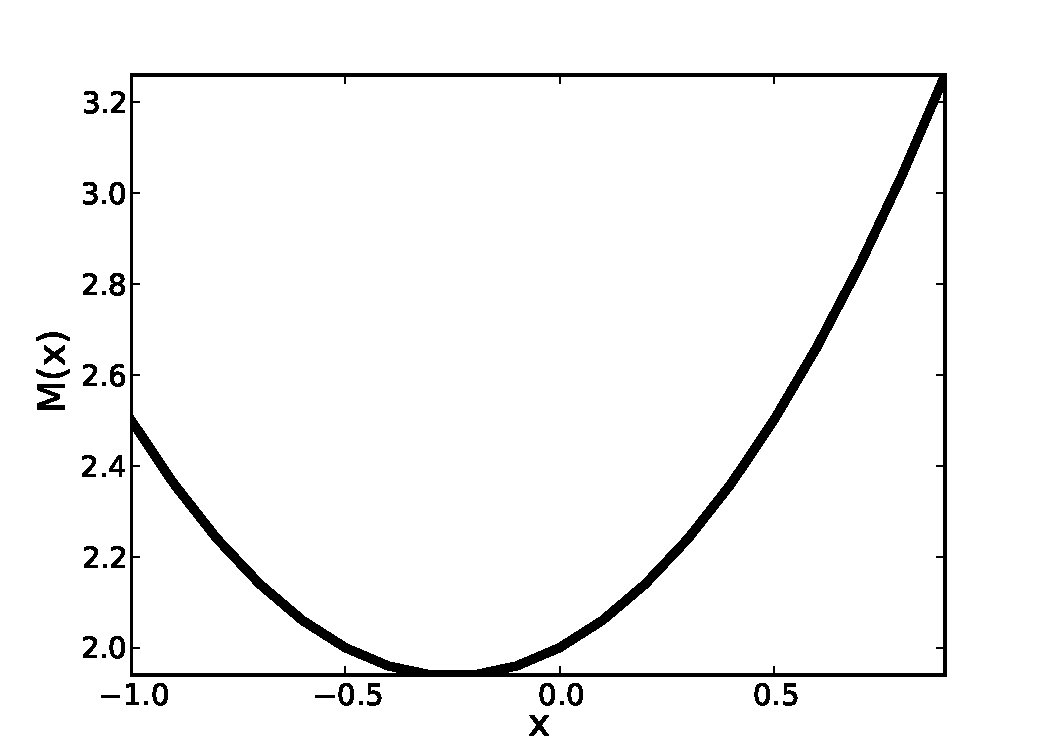
\epsfig{file=figs/mean.pdf,width=10cm}
    \caption{The mean function generated by {\sffamily `examples/mean.py'}.}
    \label{fig:mean}
\end{figure}

The first component we will create is a mean function, represented by class \class{Mean}. The mean function of a univariate GP can be interpreted as a prior guess for the GP, so it's a univariate function also. The \class{Mean} class is a wrapper for an ordinary Python function. We will use the parabolic function
\begin{equation}
    M(x) = ax^2 + bx + c.
\end{equation}

The following code will produce an instance of class \class{Mean} called M:
\verbatiminput{../../examples/gp/mean.py}

The first argument to \class{Mean}'s init method is the underlying Python function, in this case \function{quadfun}. The extra arguments \code{a}, \code{b}  and \code{c} will be memorized and passed to \function{quadfun} whenever M is called; the call \texttt{M(x)} in the plotting portion of the script doesn't need to pass them in.

Mean functions broadcast over their arguments in the same way as \citetitle[http://docs.scipy.org/doc/numpy/reference/ufuncs.html]{NumPy universal functions} \cite{numpybook}, which means that \texttt{M(x)} will return the vector
\begin{eqnarray*}
    \texttt{[M(x[0]),\ldots, M(x[N-1])]}.
\end{eqnarray*}

The last part of the code plots \texttt{M(x)} on $-1<\texttt{x}<1$, and its output is shown in figure \ref{fig:mean}. As expected, the plot is a parabola.

\subsubsection{Creating a covariance function}\label{subsub:cov}
\begin{figure}
    \centering
        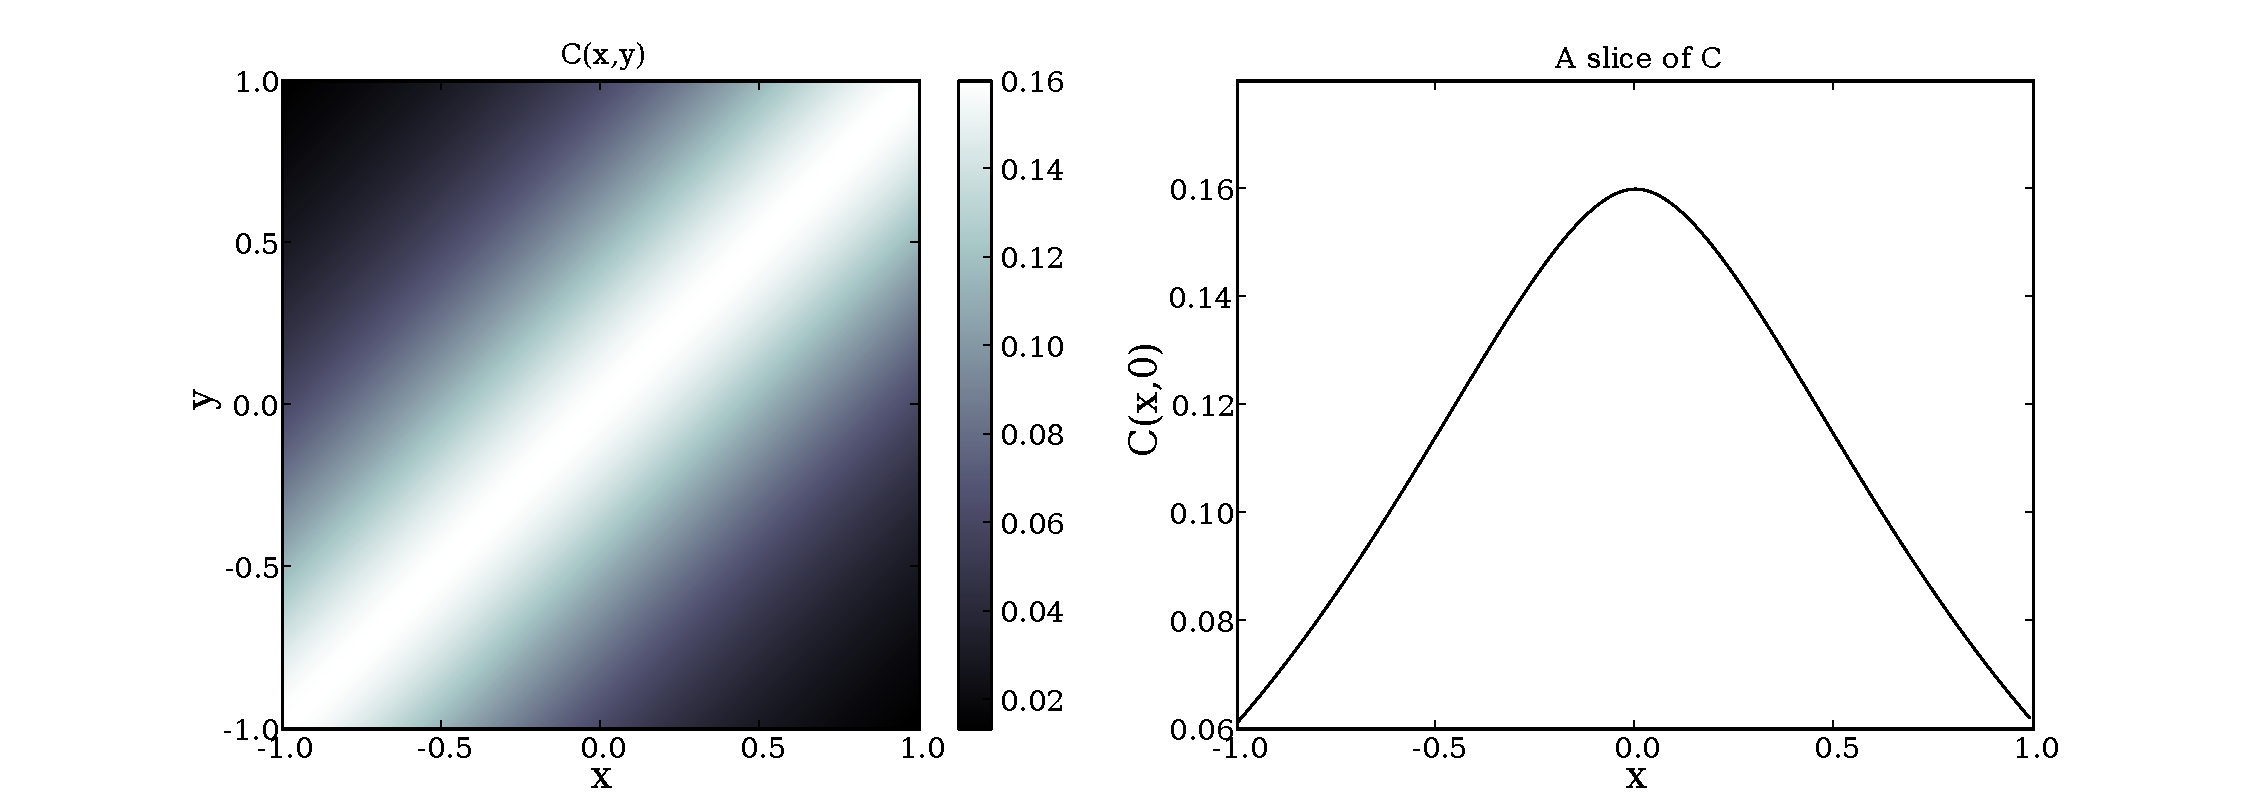
\epsfig{file=figs/cov.pdf,width=15cm}
    \caption{The covariance function generated by {\sffamily `examples/cov.py'}. On the left is the covariance function $C(x,y)$ evaluated over a square: $-1\le x\le 1,\ -1\le y\le 1$. On the right is a slice of the covariance: $C(x,0)$ for $0\le x \le 1$}
    \label{fig:cov}
\end{figure}

GP covariance functions are represented by the class \class{Covariance}, which like \class{Mean} is essentially a wrapper for ordinary Python functions. In this example we will use the popular Mat\`ern covariance function \cite{banerjee}, which is provided in module \module{cov_funs}. In addition to the two arguments \texttt{x} and \texttt{y}, this function takes three tunable parameters: \code{amp} controls the amount by which realizations may deviate from their mean, \code{diff_degree} controls the roughness of realizations (the degree of differentiability), and \code{scale} controls the lengthscale over which realizations change.

You're free to write your own functions to wrap in \class{Covariance} objects. See section \ref{cha:usercov} for more information.

The code in \file{examples/cov.py} will produce an instance of class \class{Covariance} called C.
\verbatiminput{../../examples/gp/cov.py}

The first argument to \class{Covariance}'s init method, \function{eval_fun}, gives the Python function from which the covariance function will be made. In this case, \function{eval_fun} is \function{matern.euclidean}. The extra arguments \code{diff_degree, amp} and \code{scale} will be passed to \function{matern.euclidean} every time C is called.

At this stage, the covariance function C exposes a very simple user interface. In fact, it behaves a lot like the ordinary Python function \texttt{matern.euclidean} that it wraps, except that like \texttt{Mean} it `memorizes' the parameters \code{diff_degree, amp} and \code{scale} so that you don't need to pass them in when you call it. Covariance functions' calling conventions are slightly different than ordinary numpy universal functions' \cite{numpybook}:
\begin{enumerate}
    \item Broadcasting works differently. If C were a numpy universal function, \texttt{C(x,y)} would return the following array:
    \begin{eqnarray*}
        \begin{array}{ccc}
            \texttt{[C(x[0],y[0])}& \ldots& \texttt{C(x[N-1],y[N-1])]},
        \end{array}
    \end{eqnarray*}
    where \texttt{x} and \texttt{y} would need to be vectors of the same length. In fact \texttt{C(x,y)} returns a matrix:
    \begin{eqnarray*}
        \left[\begin{array}{ccc}
            \texttt{C(x[0],y[0])}& \ldots& \texttt{C(x[0],y[Ny-1])}\\
            \vdots&\ddots&\vdots\\
            \texttt{C(x[Nx-1],y[0])}& \ldots& \texttt{C(x[Nx-1],y[Ny-1])}
        \end{array}\right],
    \end{eqnarray*}
    and input arguments \texttt{x} and \texttt{y} don't need to be the same length.
    \item You can call covariance functions with just one argument. \texttt{C(x)} returns
    \begin{eqnarray*}
         \texttt{[C(x[0],x[0])}& \ldots& \texttt{C(x[Nx-1],x[Nx-1])]} = \texttt{diag(C(x,x))},
    \end{eqnarray*}
    but is computed much faster than \texttt{diag(C(x,x))} would be.
\end{enumerate}

Most of the code in \file{examples/cov.py} is devoted to output, which is shown in figure \ref{fig:cov}. It plots the covariance function \texttt{C(x,x)} evaluated over a square, and also the `slice' \texttt{C(x,0)} over an interval. You'll notice that the graph of the full covariance function resembles a rounded A-frame tent.

\subsubsection{Drawing realizations}\label{subsub:realizations}
\begin{figure}
    \centering
        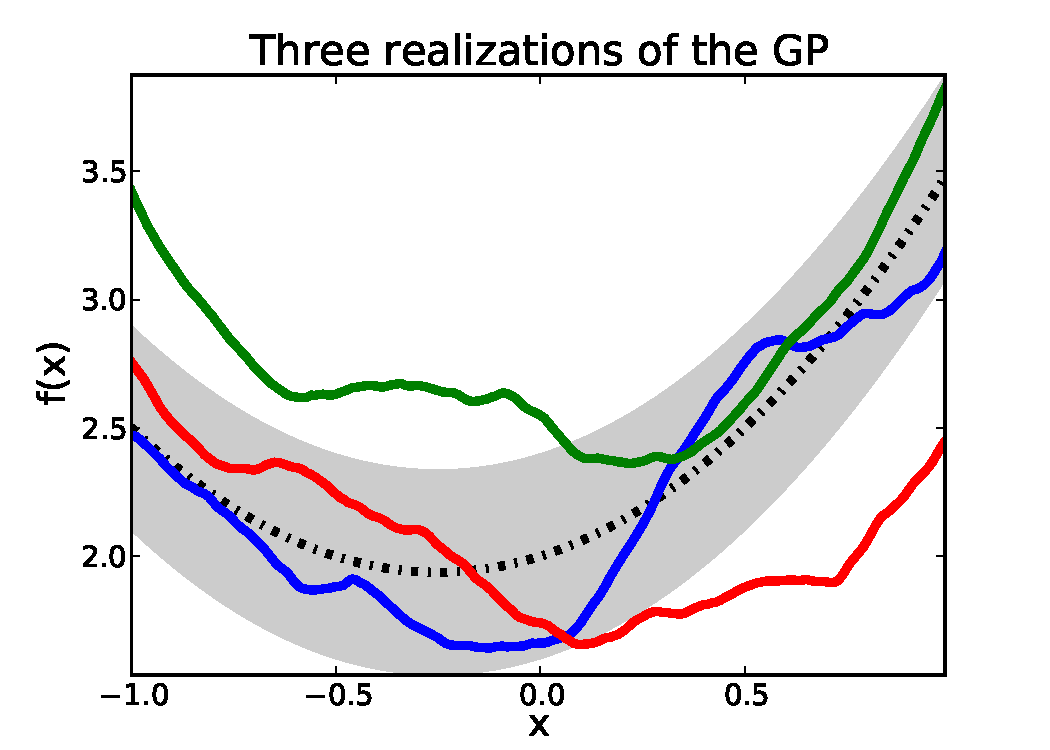
\epsfig{file=figs/realizations.pdf,width=10cm}
    \caption{Three realizations from a Gaussian process displayed with mean $\pm$ 1 sd envelope. Generated by {\sffamily `examples/realizations.py'}.}
    \label{fig:realizations}
\end{figure}

Finally, let's generate some realizations (draws) from the Gaussian process defined by M and C and take a look at them. The following code will generate a list of \class{Realization} objects:
\verbatiminput{../../examples/gp/realizations.py}

    The init method of \class{Realization} takes only two required arguments, a \class{Mean} object and a \class{Covariance} object. Each element of \code{f_list} is a Gaussian process realization, which is essentially a randomly-generated Python function. Like \class{Mean} objects, \class{Realization} objects use the same broadcasting rules as numpy universal functions. Typing \texttt{f(x)} will return the vector
\begin{eqnarray*}
    [\texttt{f(x[0])}\ldots \texttt{f(x[N-1])}].
\end{eqnarray*}


The plotting portion of the code calls the function \function{plot_envelope}, which summarizes some aspects of the distribution. The dashdot black line in the middle is $M$, and the gray band is the $\pm 1$ standard deviation envelope for $f$, generated by $C$. Each of the three realizations in \texttt{f_list} is a callable function, and they are plotted superimposed on the envelope. The plot output is shown in figure \ref{fig:realizations}.


\section{The role of the covariance function}\label{sec:cov}
The following covariance functions for Euclidean coordinates are included in the module \module{cov_funs}:
\begin{itemize}
    \item \texttt{matern.euclidean}
    \item \texttt{sphere.euclidean}
    \item \texttt{pow_exp.euclidean}
    \item \texttt{gaussian.euclidean}
    \item \texttt{quadratic.euclidean}
\end{itemize}
See section 2.1.3 of \citetitle[http://www.statsnetbase.com/ejournals/books/book_summary/summary.asp?id=1285]{Banerjee et al.} \cite{banerjee} for more information on each of these. Each covariance function takes at least two parameters, called \texttt{amp} and \texttt{scale}. The following covariance functions take extra parameters:
\begin{description}
    \item[\texttt{matern}:] \texttt{diff_degree}
    \item[\texttt{pow_exp}:] \texttt{pow}
    \item[\texttt{quadratic}:] \texttt{phi}.
\end{description}

In this section we'll focus on the Mat\`ern family, as it is generally considered the state of the art. Its popularity is due to the fact that it has three parameters, each of which clearly controls one of three important properties of realizations: roughness, lengthscale of changes and amplitude.

In this section we'll set the mean function to zero (more precisely, a function whose output value is zero regardless of input) in order to focus on the covariance. This:
\begin{eqnarray*}
    f\sim\textup{GP}(M,C)
\end{eqnarray*}
is equivalent to this:
\begin{eqnarray*}
    f = M + g, \\g\sim \textup{GP}(0,C),
\end{eqnarray*}
so it's not difficult to adapt the intuition we gain in this section to GPs with nontrivial mean functions.

The covariance functions listed above are \emph{stationary} and \emph{isotropic}. Intuitively, that means our a priori expectation of how $f$ will deviate from its mean doesn't vary with location or with the direction in which we look (for functions of several variables). Section \ref{cha:usercov} describes how these restrictions can be relaxed.

All the figures in this section were produced using the file \file{examples/cov_params.py}. You can follow along by editing the line of that file which reads
\begin{verbatim}
C = Covariance(eval_fun = matern.euclidean, diff_degree = 1.4, amp = 1., scale = 1.)
\end{verbatim}

The actual formulas for the covariance functions are given in section \ref{cha:usercov}, but the Mat\`ern formula is fairly inscrutable (though its Fourier transform is much more readable \cite{stein}). This section will try to help you understand it graphically.

\subsection*{The \texttt{amp} and \texttt{scale} parameters}\label{sub:ampscale}

These parameters are common to all covariance functions provided by this package, not just \texttt{matern.euclidean}. Please see section \ref{cha:usercov} if you're planning on writing your own covariance functions, as this package provides utilities that will endow them with these parameters.

As mentioned in section \ref{subsub:cov}, the covariance function plotted in figure \ref{fig:cov} resembles a rounded A-frame tent. The width of this tent controls how tightly nearby evaluations of a realization $f$ will be coupled to each other. If the tent is wide, $f(x)$ and $f(y)$ will tend to have similar values when $x$ and $y$ are close to one another. If the tent is narrower, $f(x)$ and $f(y)$ won't be as tightly correlated. The height of the tent controls the overall amplitude of $f$'s deviation from its mean.

The mathematical definition of the covariance function is as follows:
\begin{equation}
    \label{covdef}
    C(x,y)=\textup{cov}(f(x), f(y)).
\end{equation}
That implies the following:
\begin{eqnarray*}
    \textup{var}(f(x))=C(x,x).
\end{eqnarray*}
By the definition of variance, for any real number $a$
\begin{eqnarray*}
    \textup{var}( a f(x))=a^2 C(x,x).
\end{eqnarray*}

The covariance function is multiplied by \texttt{amp}$^\texttt{2}$, and this effectively multiplies realizations by \texttt{amp}. In other words, a larger \texttt{amp} parameter means that realizations will deviate further from their mean. The effects of changing the \texttt{amp} parameter are illustrated in figure \ref{fig:amp}.
\begin{figure}
    \centering
        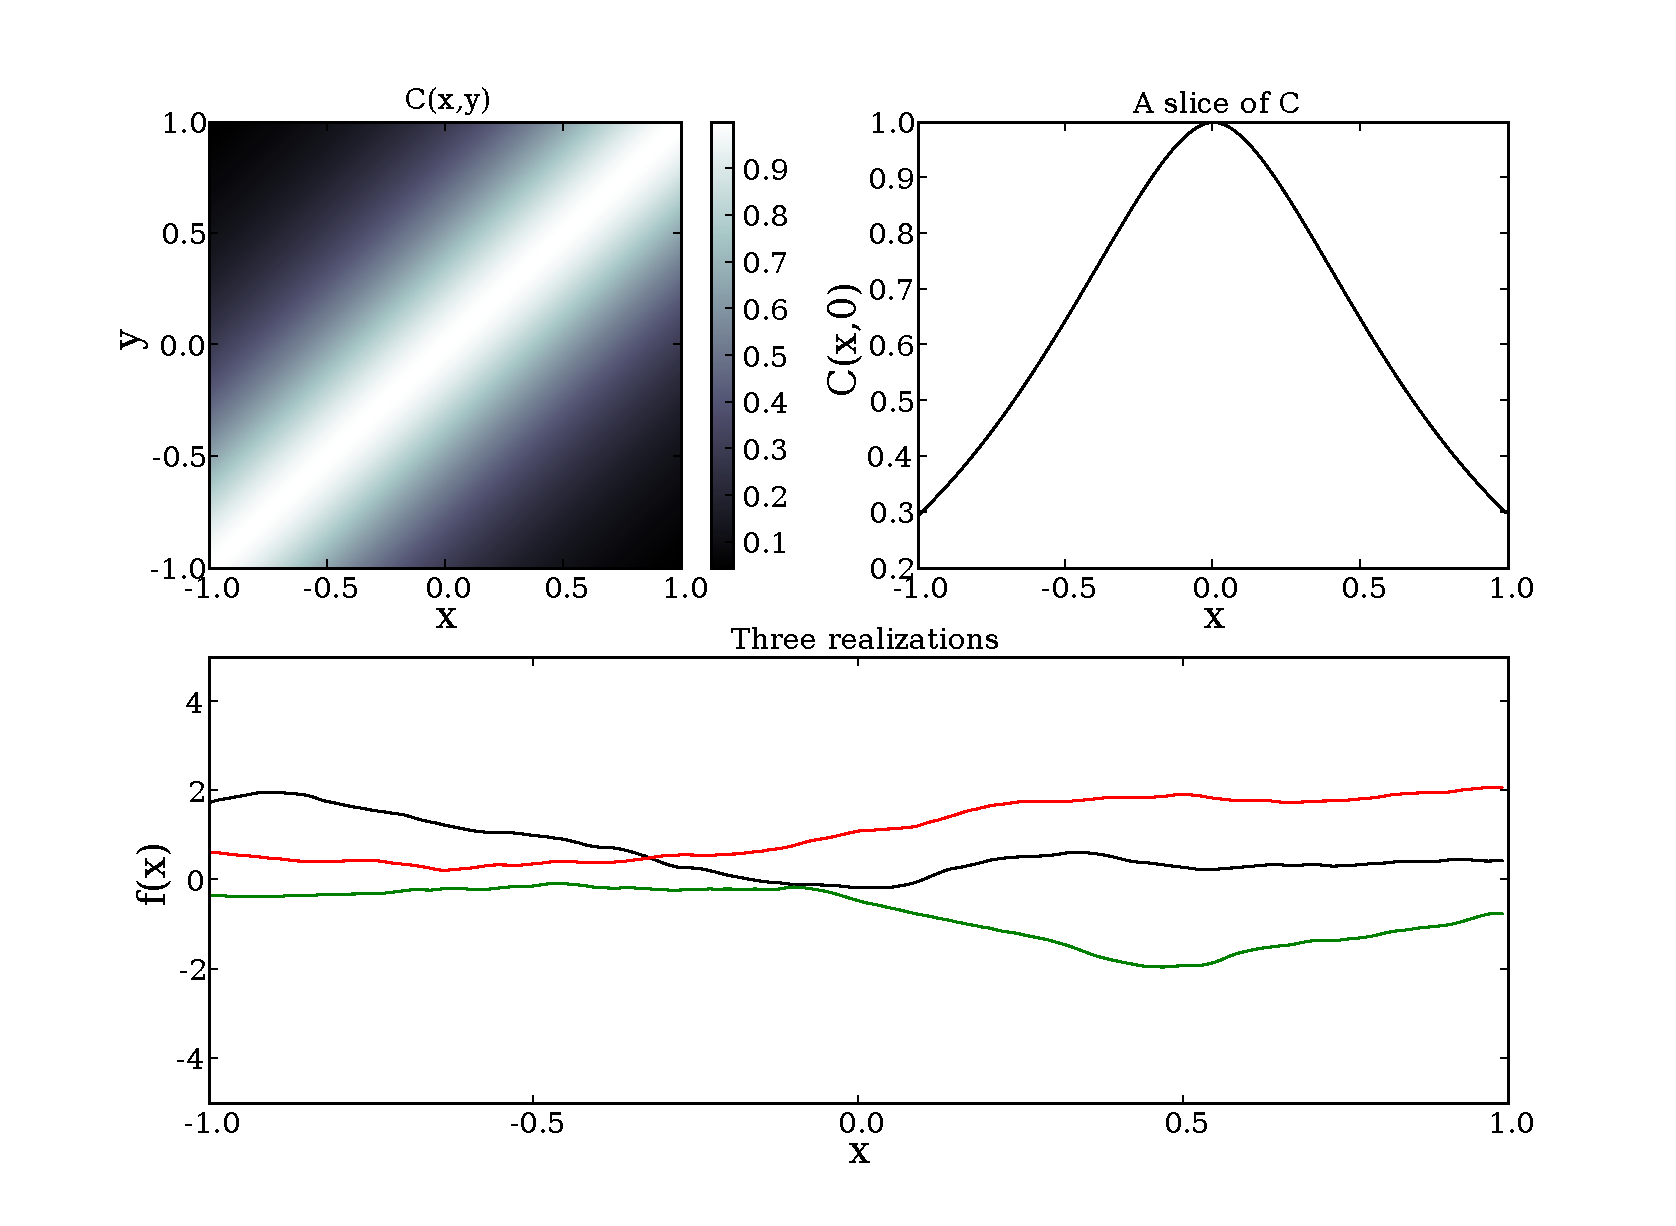
\epsfig{file=figs/d14a1s1.pdf, width=8cm}
        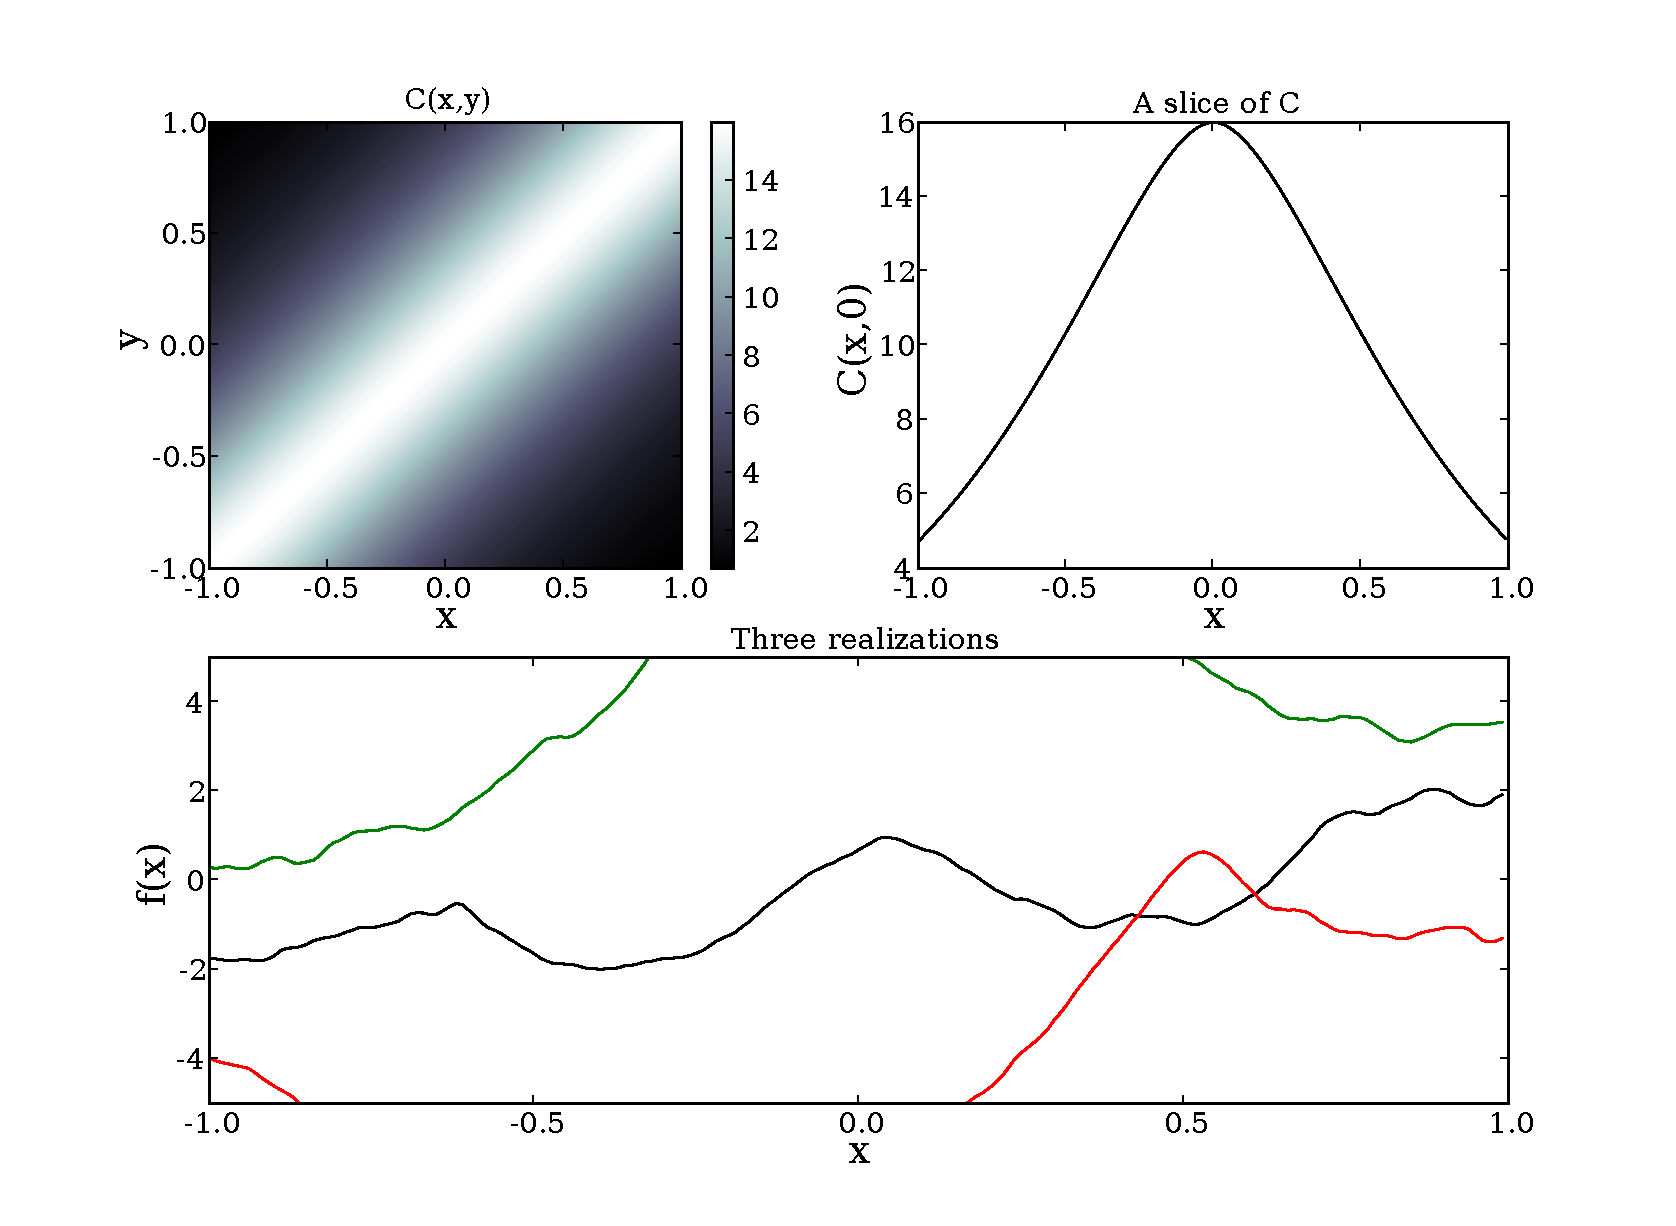
\epsfig{file=figs/d14a4s1.pdf, width=8cm}
    \caption{Mat\`ern covariances with \texttt{diff_degree=1.4}, \texttt{scale=1}, and \texttt{amp=1} (left) and 4 (right), and corresponding realizations. The amplitude of realizations tends to scale with \texttt{amp}, and the amplitude of the covariance function scales with \texttt{amp}$^2$. Note the scales on the plots of the covariance functions.}
    \label{fig:amp}
\end{figure}

Say $C$'s value can be computed from the difference in its arguments, $x-y$, rather than the arguments themselves. In that case, substituting $(x-y)/s$ for $x-y$, where $s$ is greater than 1, will make the input points `appear' closer together.

Whenever a call $C(x,y)$ is made, the distances between elements of the input arrays $x$ and $y$ are divided by the \texttt{scale} parameter before being passed to the underlying covariance function. In our one-dimensional example this effectively stretches the realizations in the $x$ direction. If \texttt{scale} is large, the function will be correlated over a larger distance and will not `wiggle' as quickly. Figure \ref{fig:scale} illustrates the effects of the scale parameter.
\begin{figure}
    \centering
        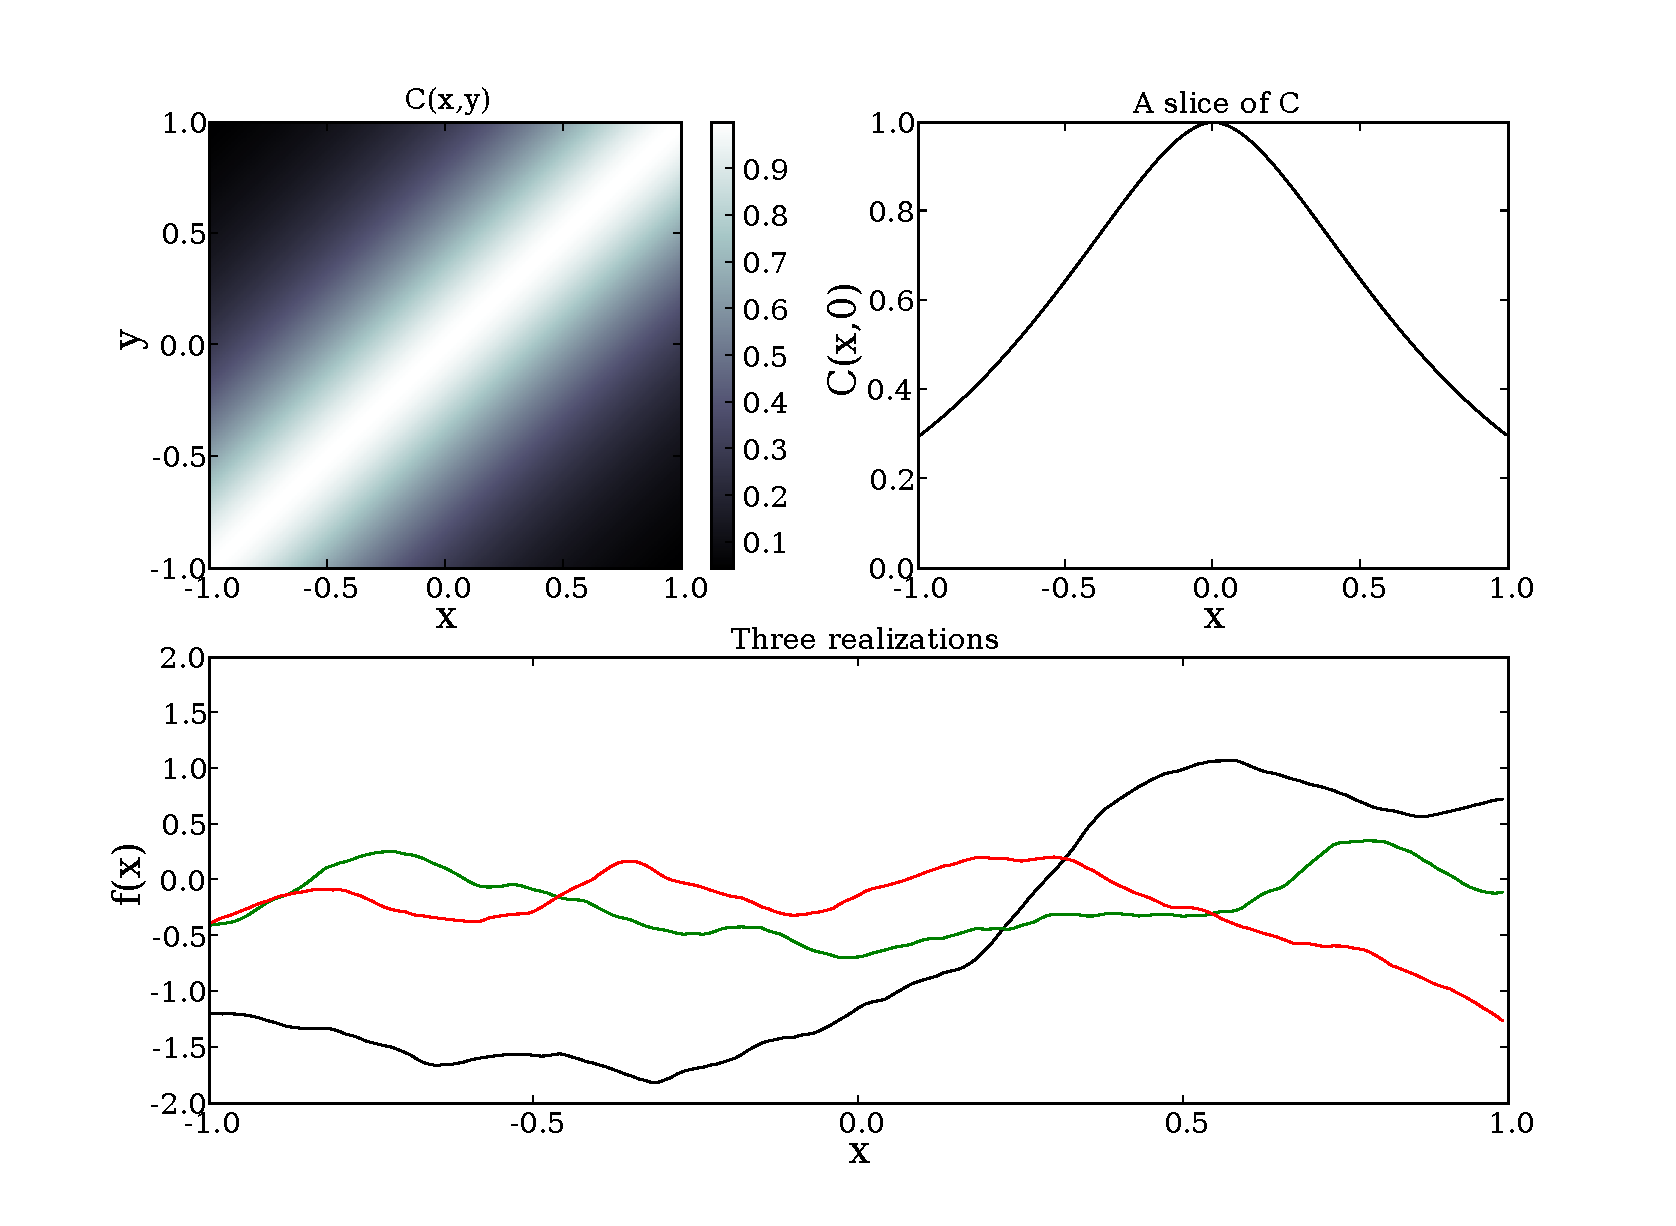
\epsfig{file=figs/d14a1s1close.pdf, width=5cm}
        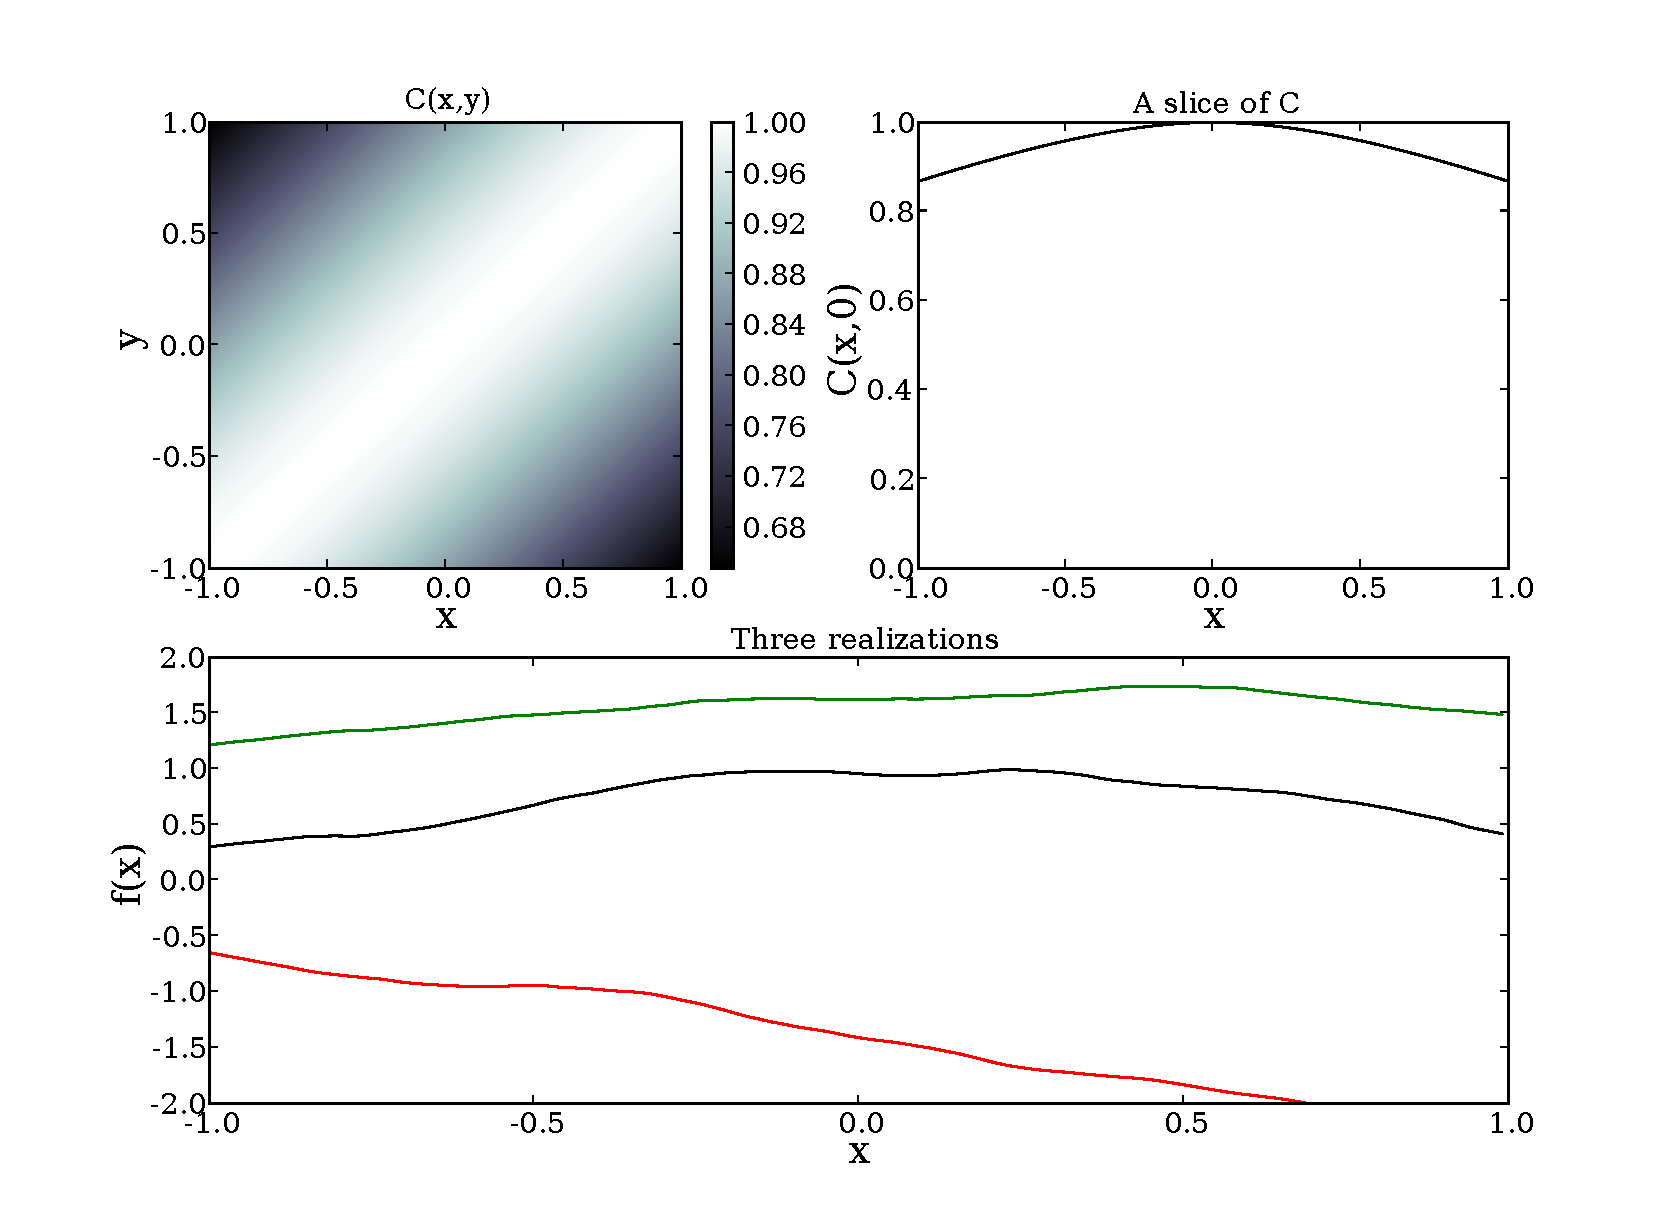
\epsfig{file=figs/d14a1s4.pdf, width=5cm}
        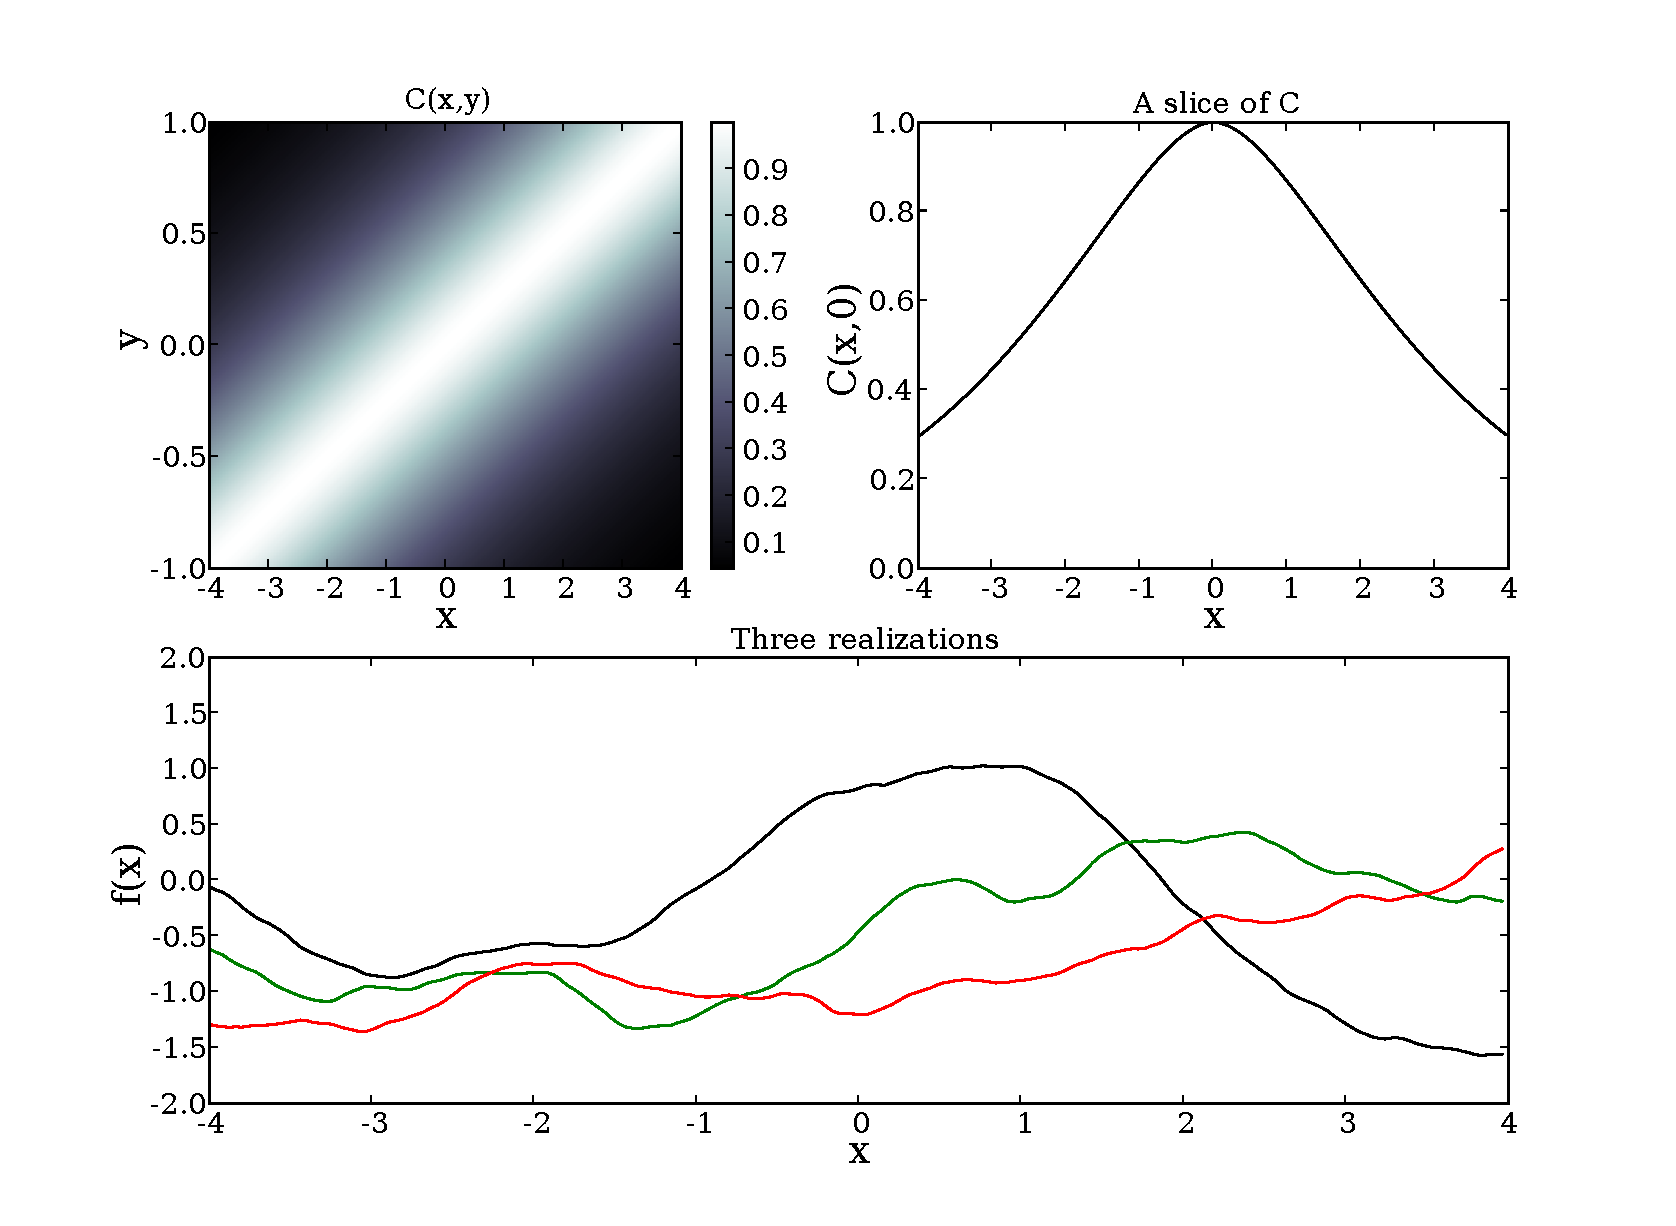
\epsfig{file=figs/d14a1s4far.pdf, width=5cm}
    \caption{Mat\`ern covariances with \texttt{diff_degree=1.4}, \texttt{amp=1} and \texttt{scale=1} (left) and \texttt{scale=4} (center, right), and corresponding realizations. A larger value of \texttt{scale} stretches both covariance functions and realizations (center), so that realizations don't wiggle as rapidly. When the stretched functions are plotted on commensurately stretched axes (right), they look like the unstretched functions again.}
    \label{fig:scale}
\end{figure}

\subsection{The \texttt{diff_degree} parameter}\label{sub:diffdegree}
The \texttt{diff_degree} parameter, usually denoted $\nu$, is unique (amongst the covariance functions provided by this package) to the Mat\`ern family of covariance functions. It controls the sharpness of the ridge of the covariance function, which controls the roughness/smoothness of realizations.

More specifically, look at the slices $C(x,0)$ that are shown in the upper right-hand panels of the subfigures in figures \ref{fig:amp} and \ref{fig:scale}. If \texttt{diff_degree} is greater than an integer $n$, this slice is $2n$ times differentiable at $x=0$. It turns out that this means realizations will be $n$ times differentiable.

It's natural to ask what happens when \texttt{diff_degree} isn't an integer. There is such a thing as \citetitle[http://en.wikipedia.org/wiki/Fractional_calculus]{fractional calculus}, which deals with things like taking half a derivative. Stein \cite{stein} discusses the connection briefly. See also Miller and Ross \cite{fraccalc}.

For our purposes, it's safe to say that \texttt{diff_degree} is a roughness index that can be interpreted as a degree of differentiability when it is an integer. Figure \ref{fig:diffdegree} illustrates the effects of changing this parameter:
\begin{description}
    \item[0 (not shown):] $C(x,y)=1$ if $y=x$, $0$ if $\texttt{x}\ne \texttt{y}$. Not only are realizations not differentiable, they're not even continuous. $f(x)$ is an independent normal random variable for each value of $x$.
    \item[.2:] $C(x,0)$ is not even one time differentiable at its peak, where $x=0$. Realizations are very rough, but continuous.
    \item[.5:] If \texttt{diff_degree} is just larger than $.5$, $C(x,0)$ is differentiable at $x=0$. Realizations, however, aren't differentiable; their roughness is comparable to trajectories of Brownian particles. When \texttt{diff_degree} is equal to \texttt{.5}, \texttt{matern} is equivalent to another covariance function, \texttt{pow_exp}, with extra argument \texttt{pow=1}.
    \item[1:] If \texttt{diff_degree} is just larger than $1$, $C(x,0)$ is twice differentiable at $x=0$, and realizations are differentiable.
    \item[1.4:] The value from figures \ref{fig:amp}, \ref{fig:cov} and \ref{fig:scale} is shown for comparison.
    \item[2:] If \texttt{diff_degree} is just larger than $2$, $C(x,0)$ is four times differentiable at $x=0$, and realizations are twice differentiable.
    \item[10:] Realizations are very smooth. As \texttt{diff_degree} approaches infinity, \texttt{matern} gets closer to \texttt{gaussian}. Realizations from GPs with Gaussian covariances are infinitely differentiable. In fact, if \texttt{diff_degree} is larger than 10 \texttt{matern} simply calls \texttt{gaussian}, because it's much faster. 
\end{description}

\begin{figure}
    \centering
        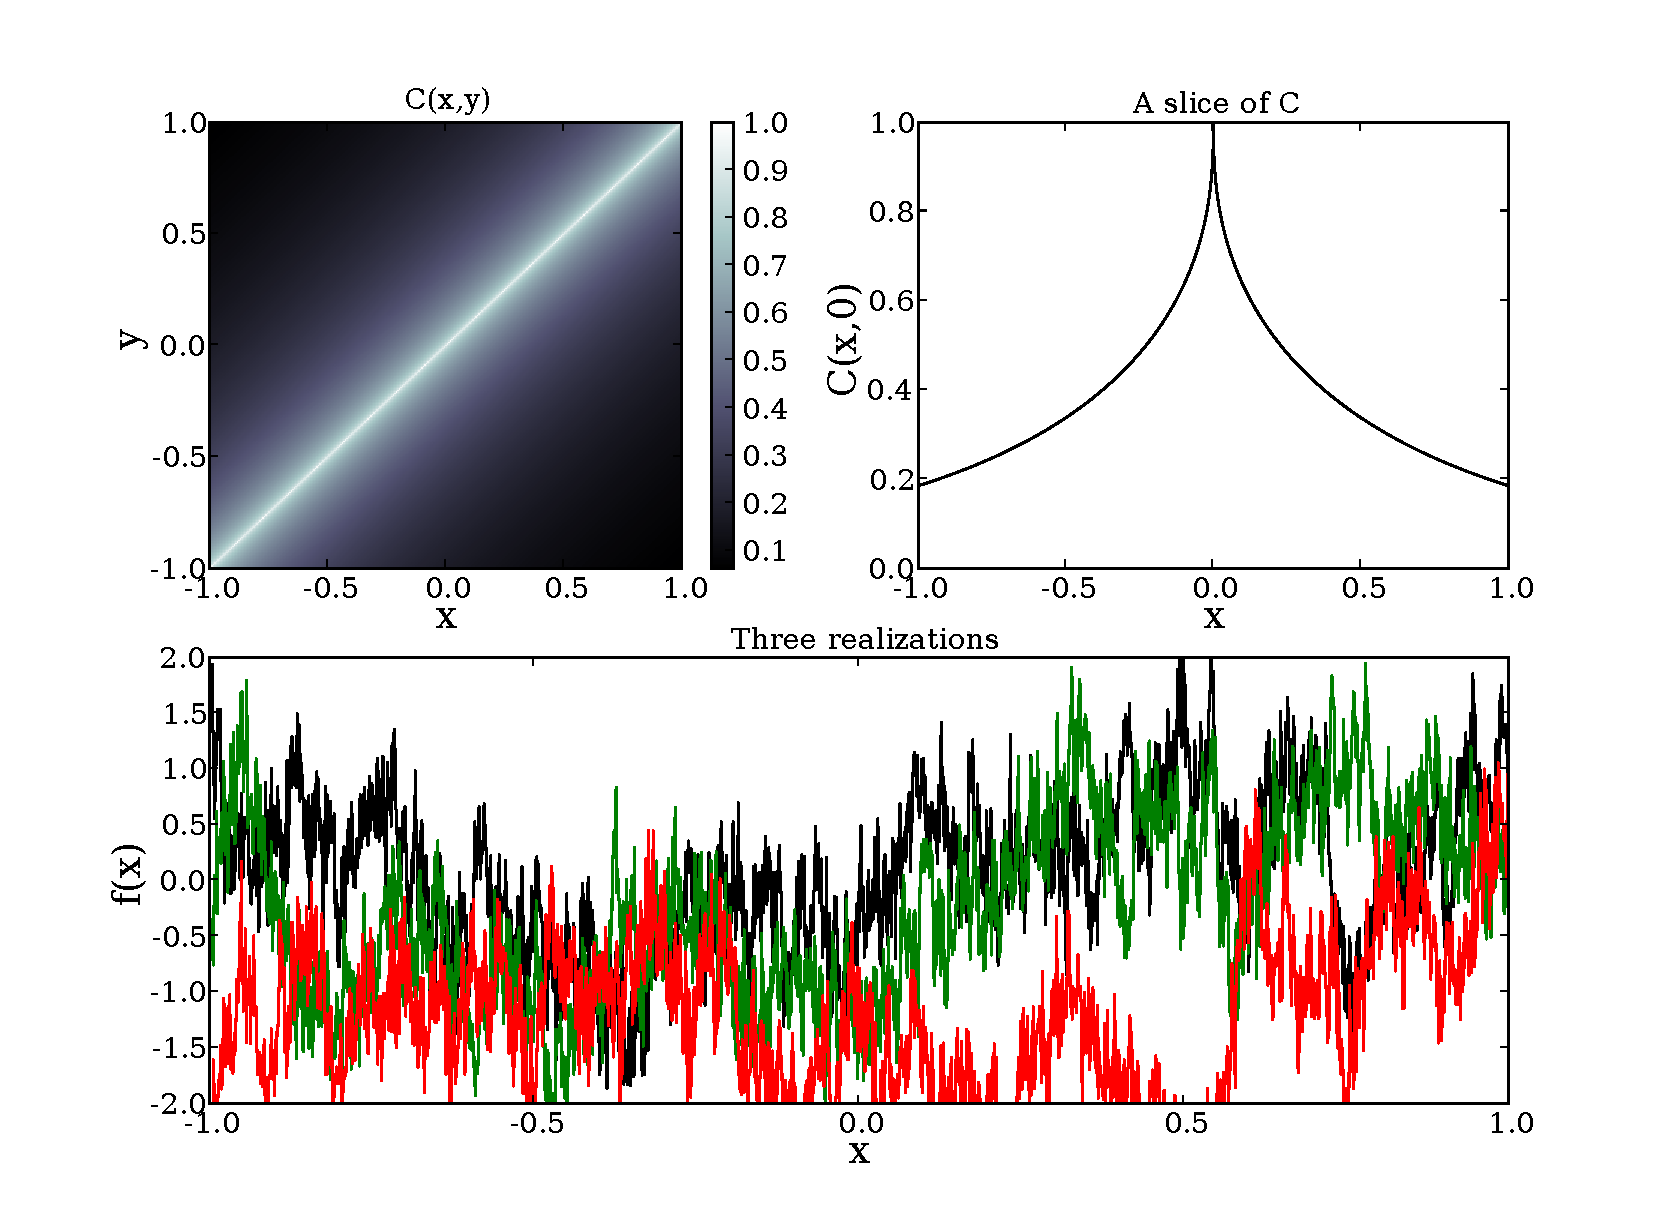
\epsfig{file=figs/d2a1s1.pdf,width=8cm}
        % 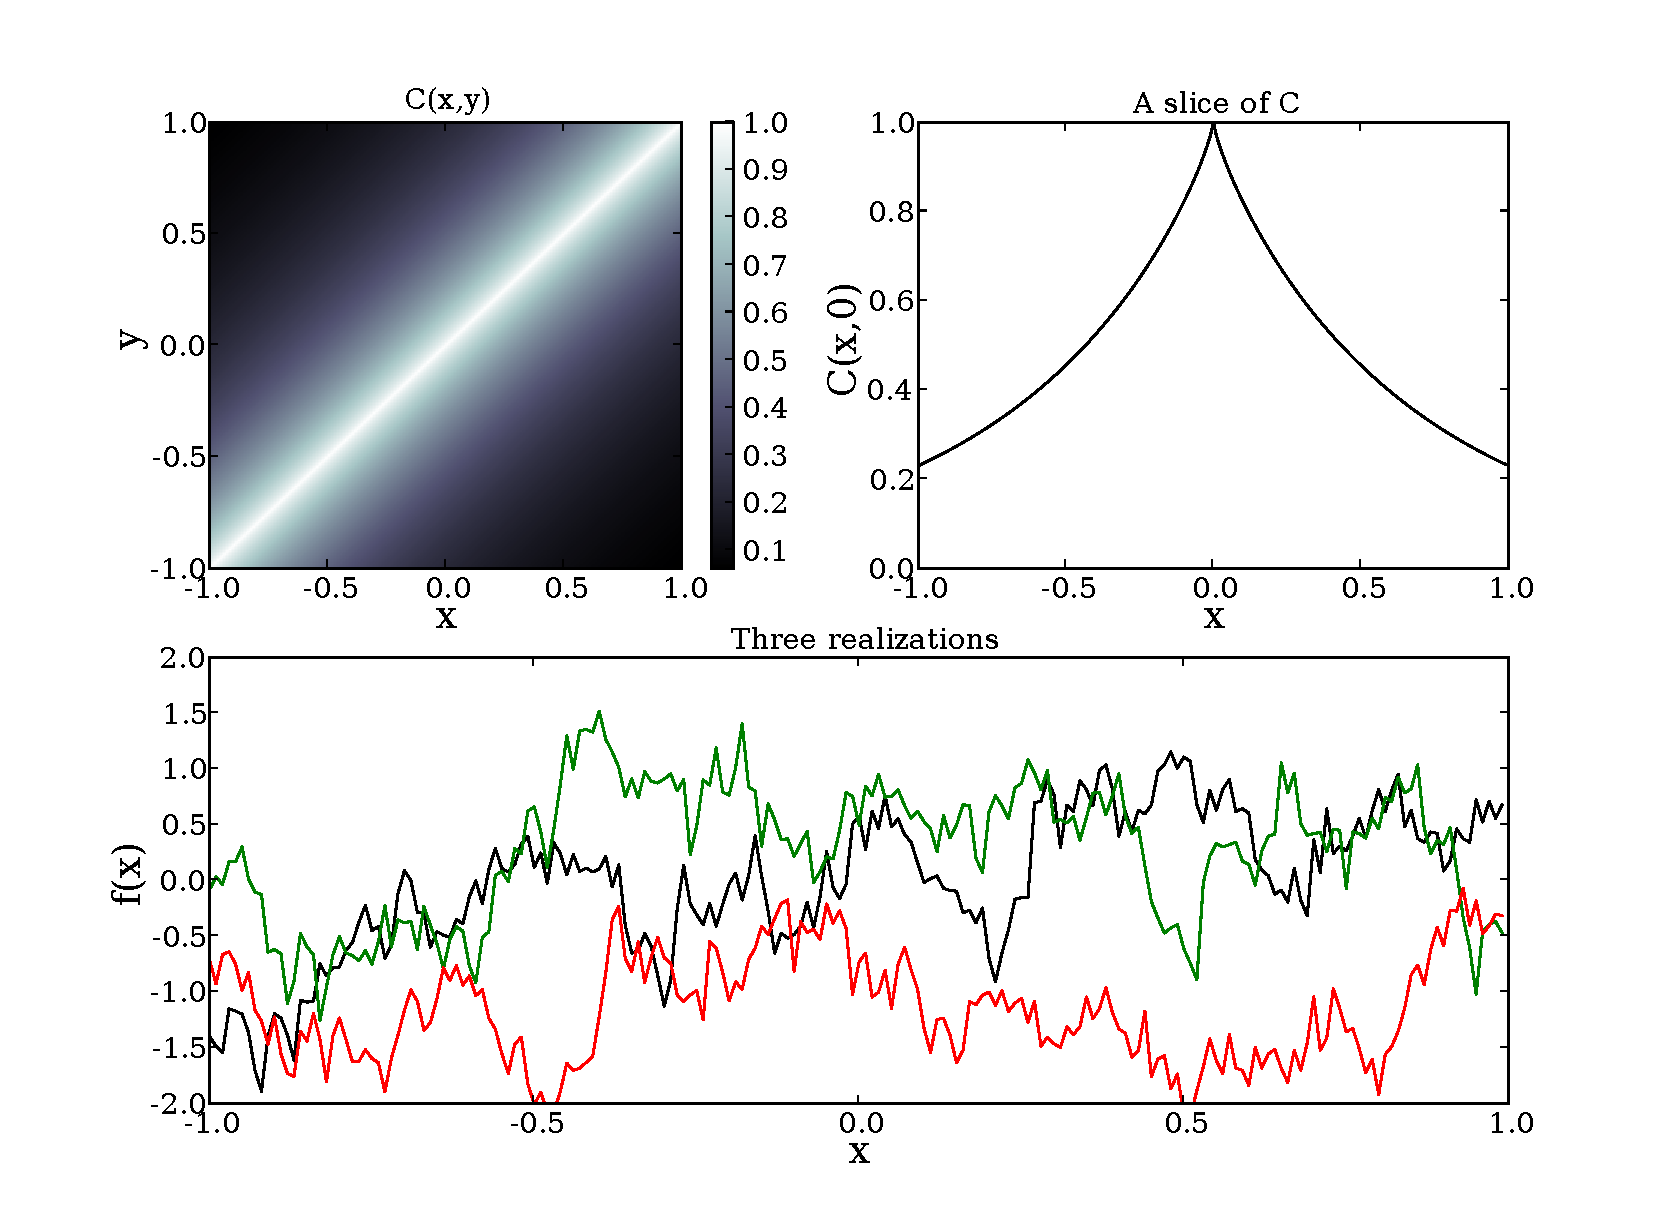
\epsfig{file=figs/d4a1s1.pdf,width=4cm}
        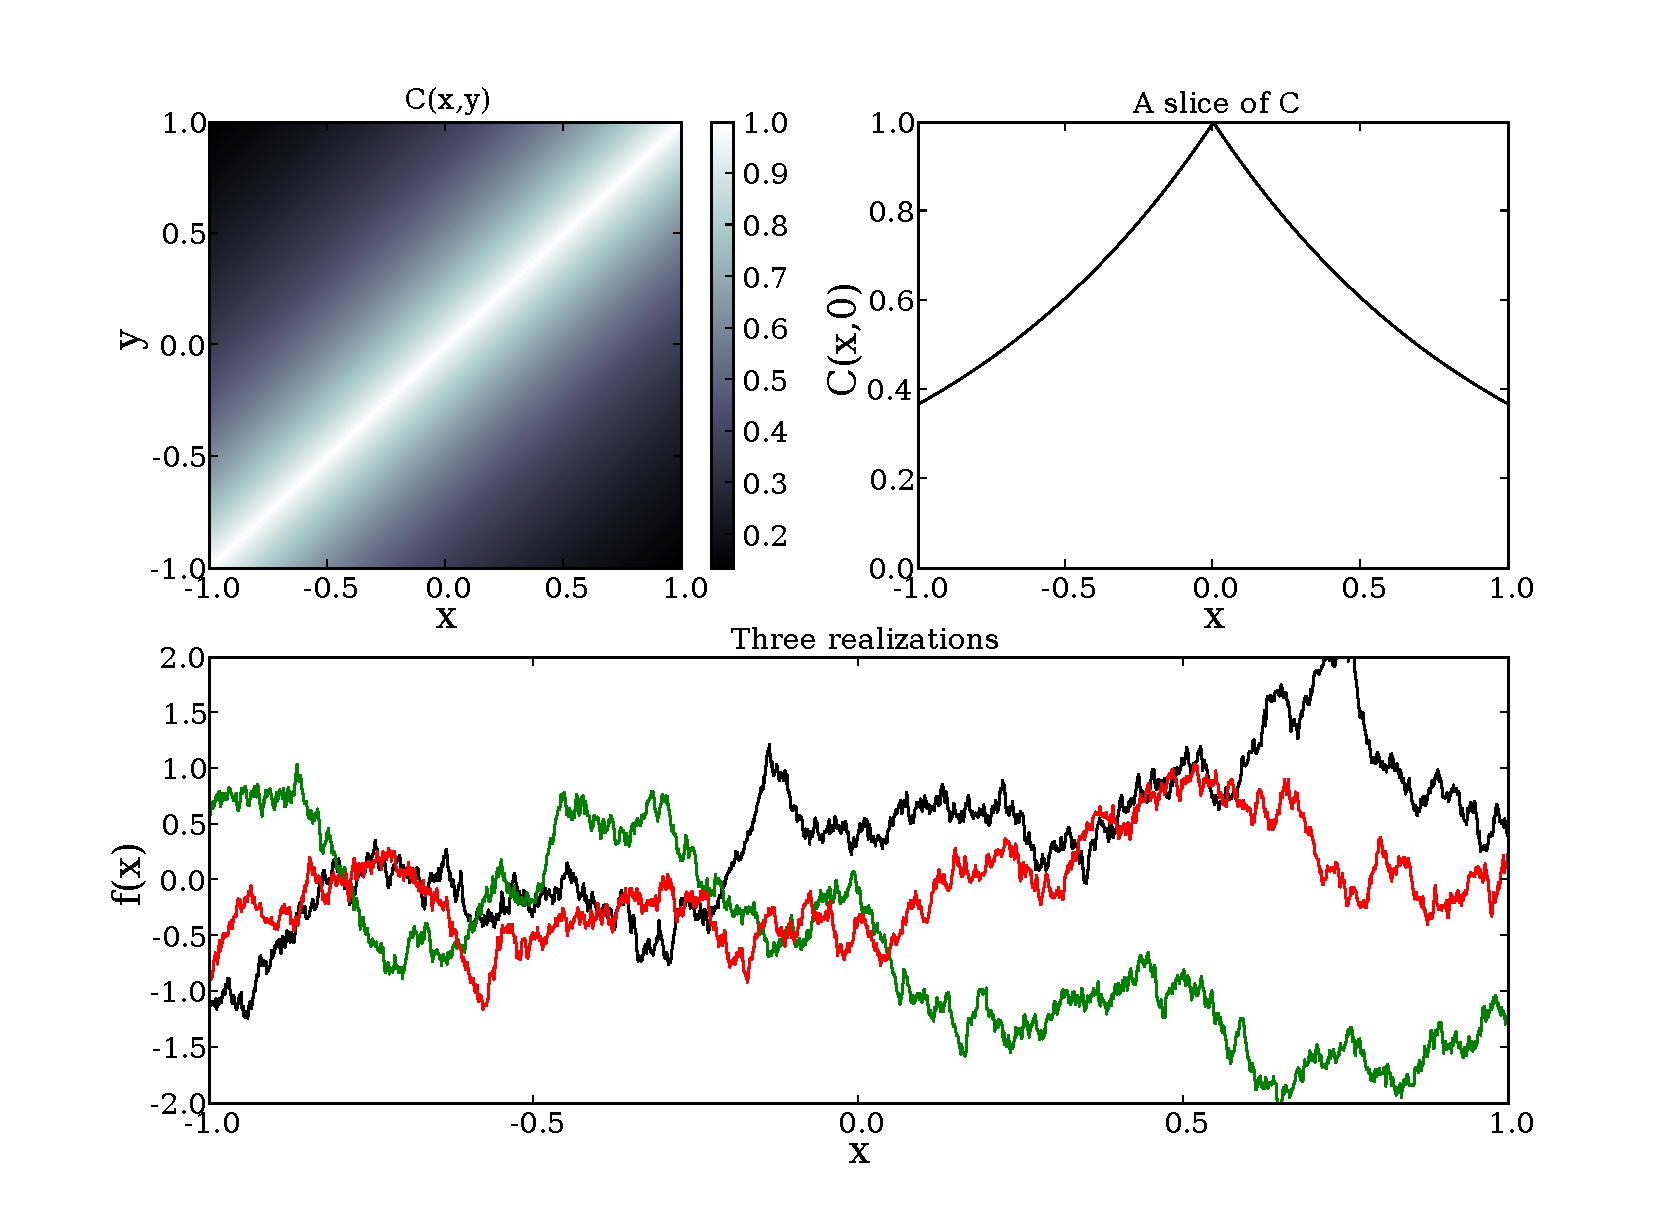
\epsfig{file=figs/d5a1s1.pdf,width=8cm}
        % 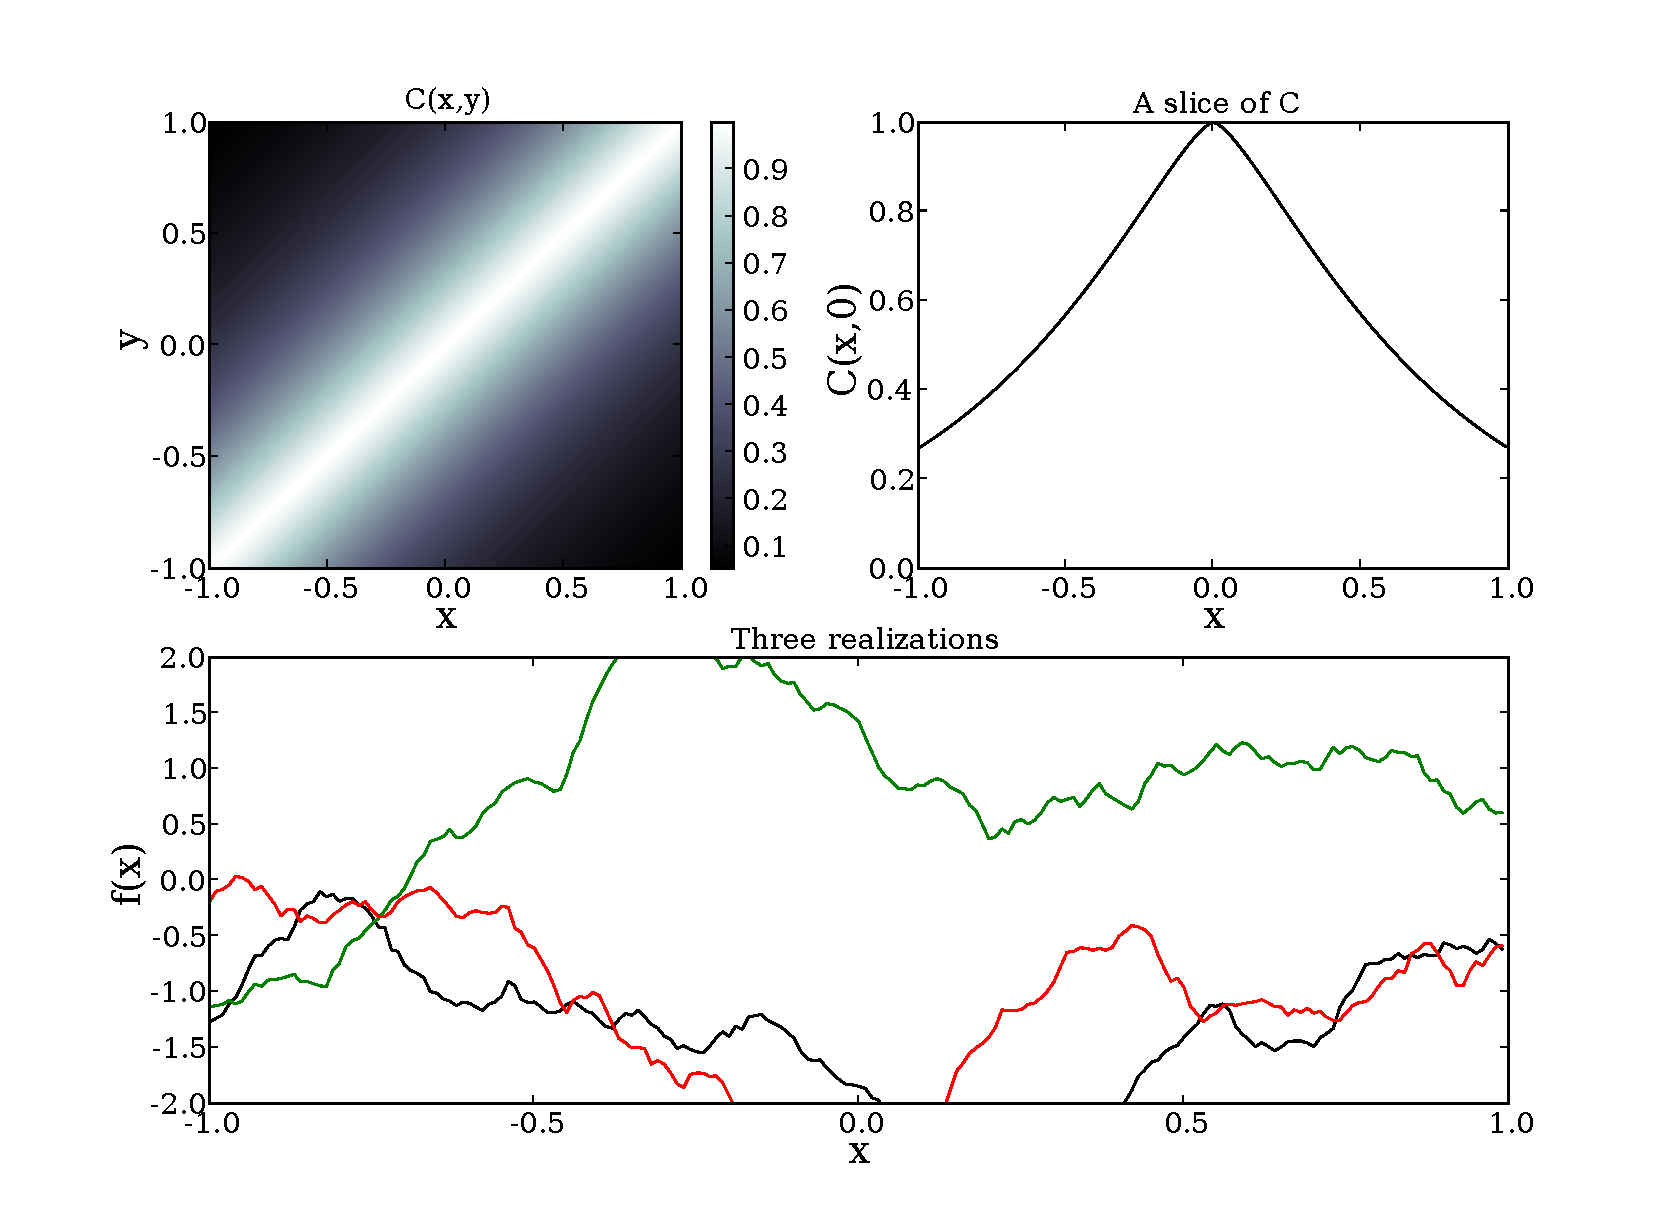
\epsfig{file=figs/d8a1s1.pdf,width=4cm}
        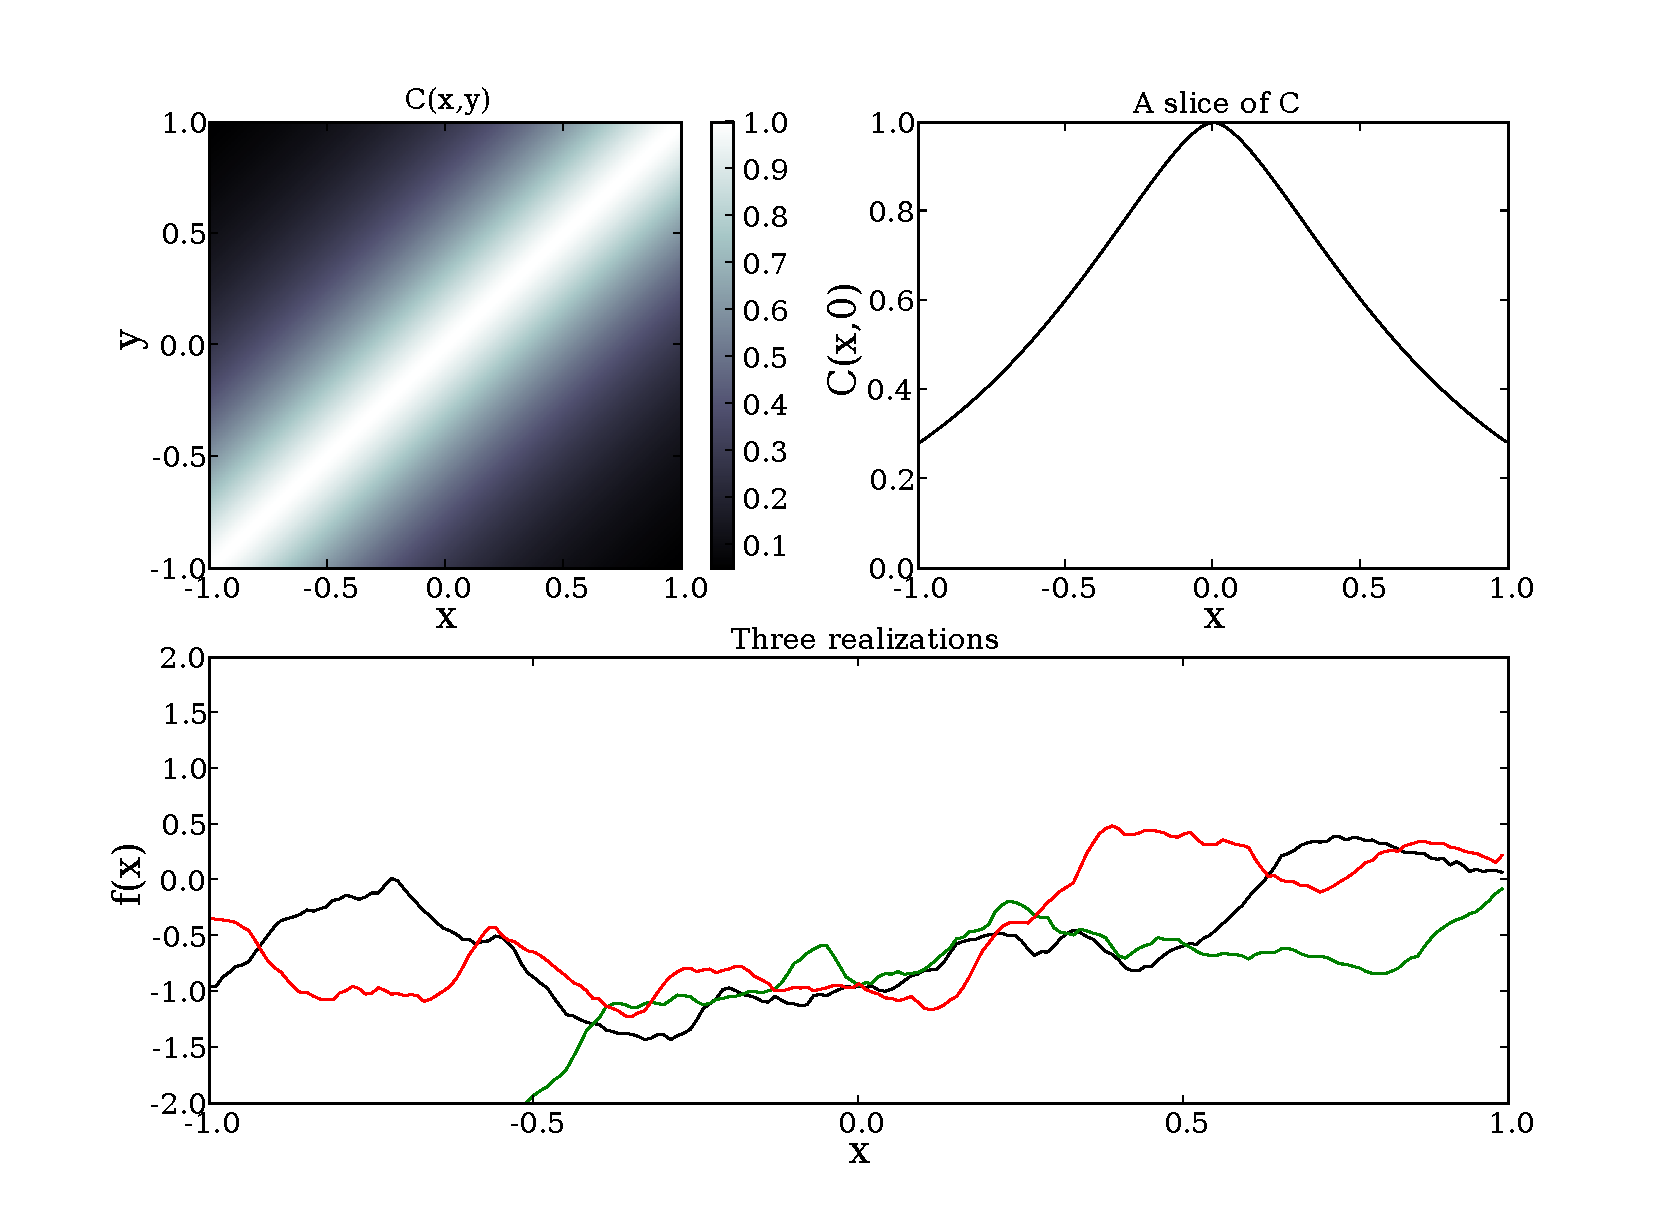
\epsfig{file=figs/d10a1s1.pdf,width=8cm}
        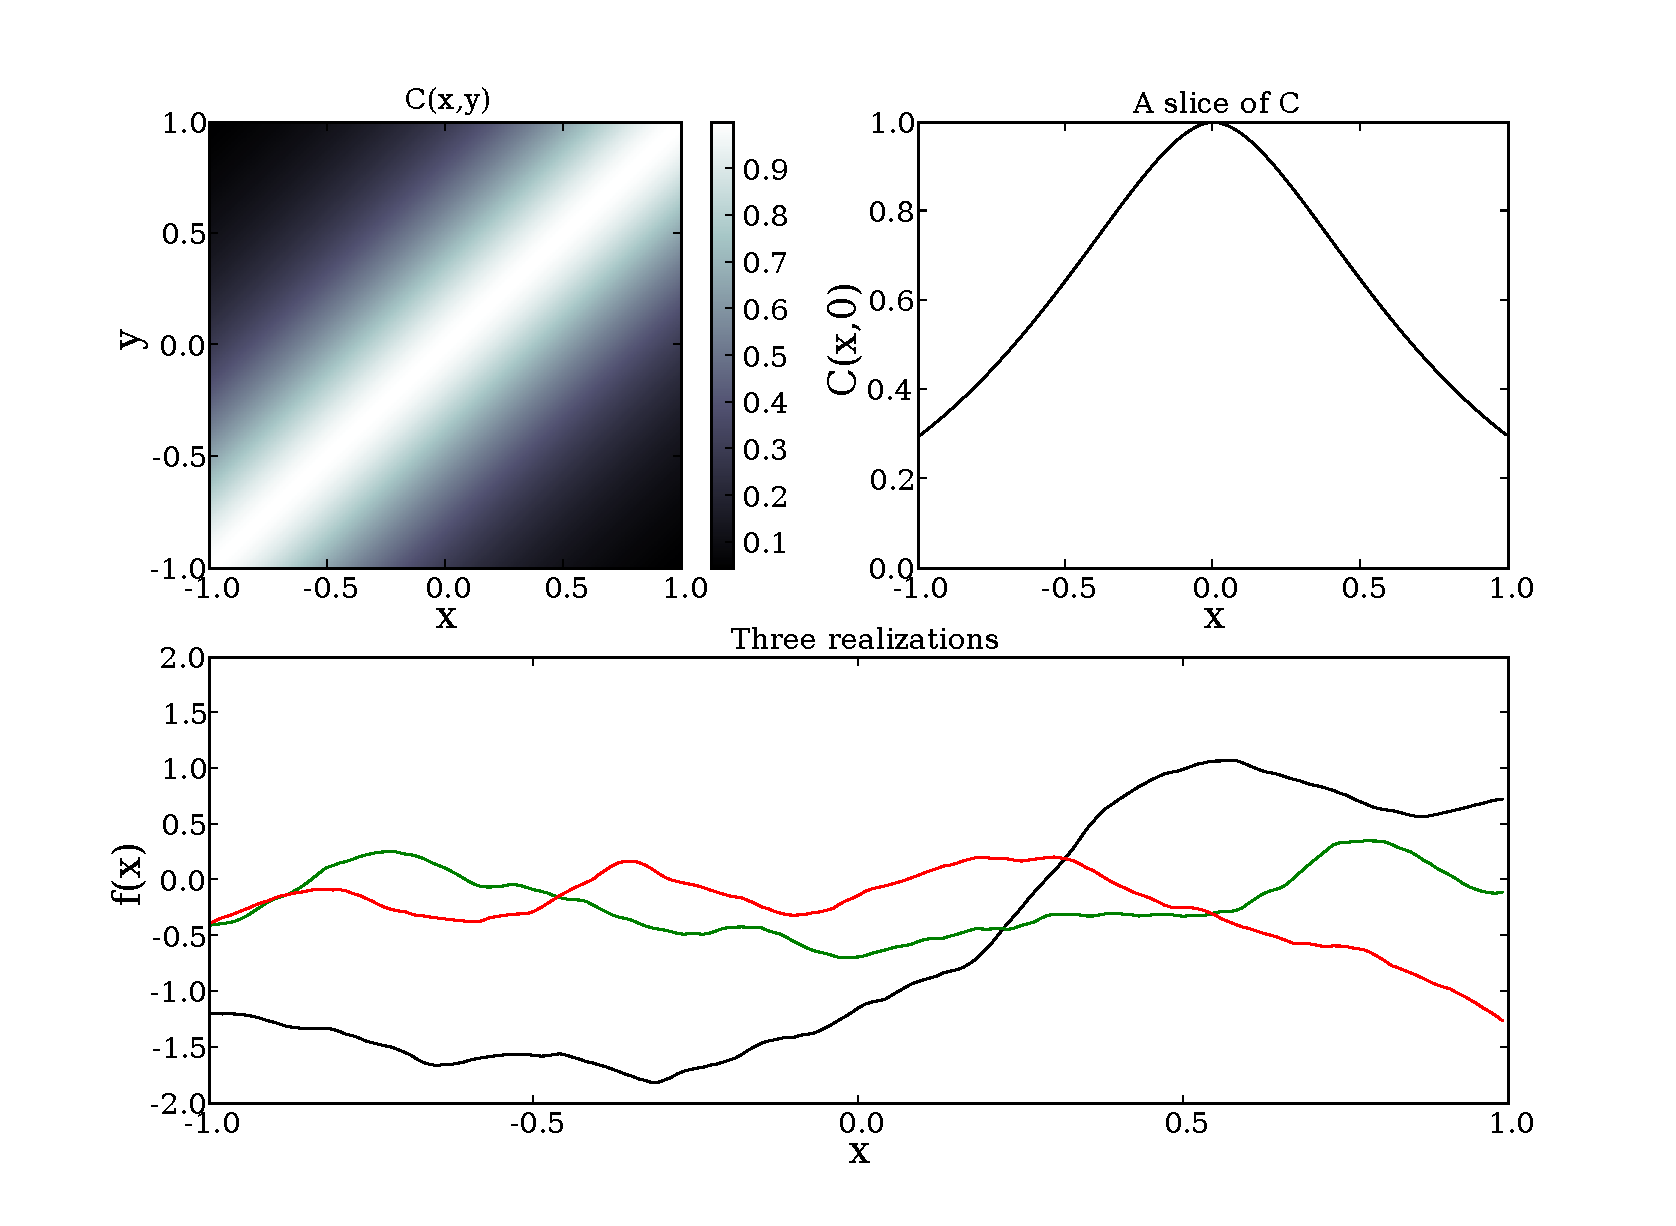
\epsfig{file=figs/d14a1s1close.pdf,width=8cm}
        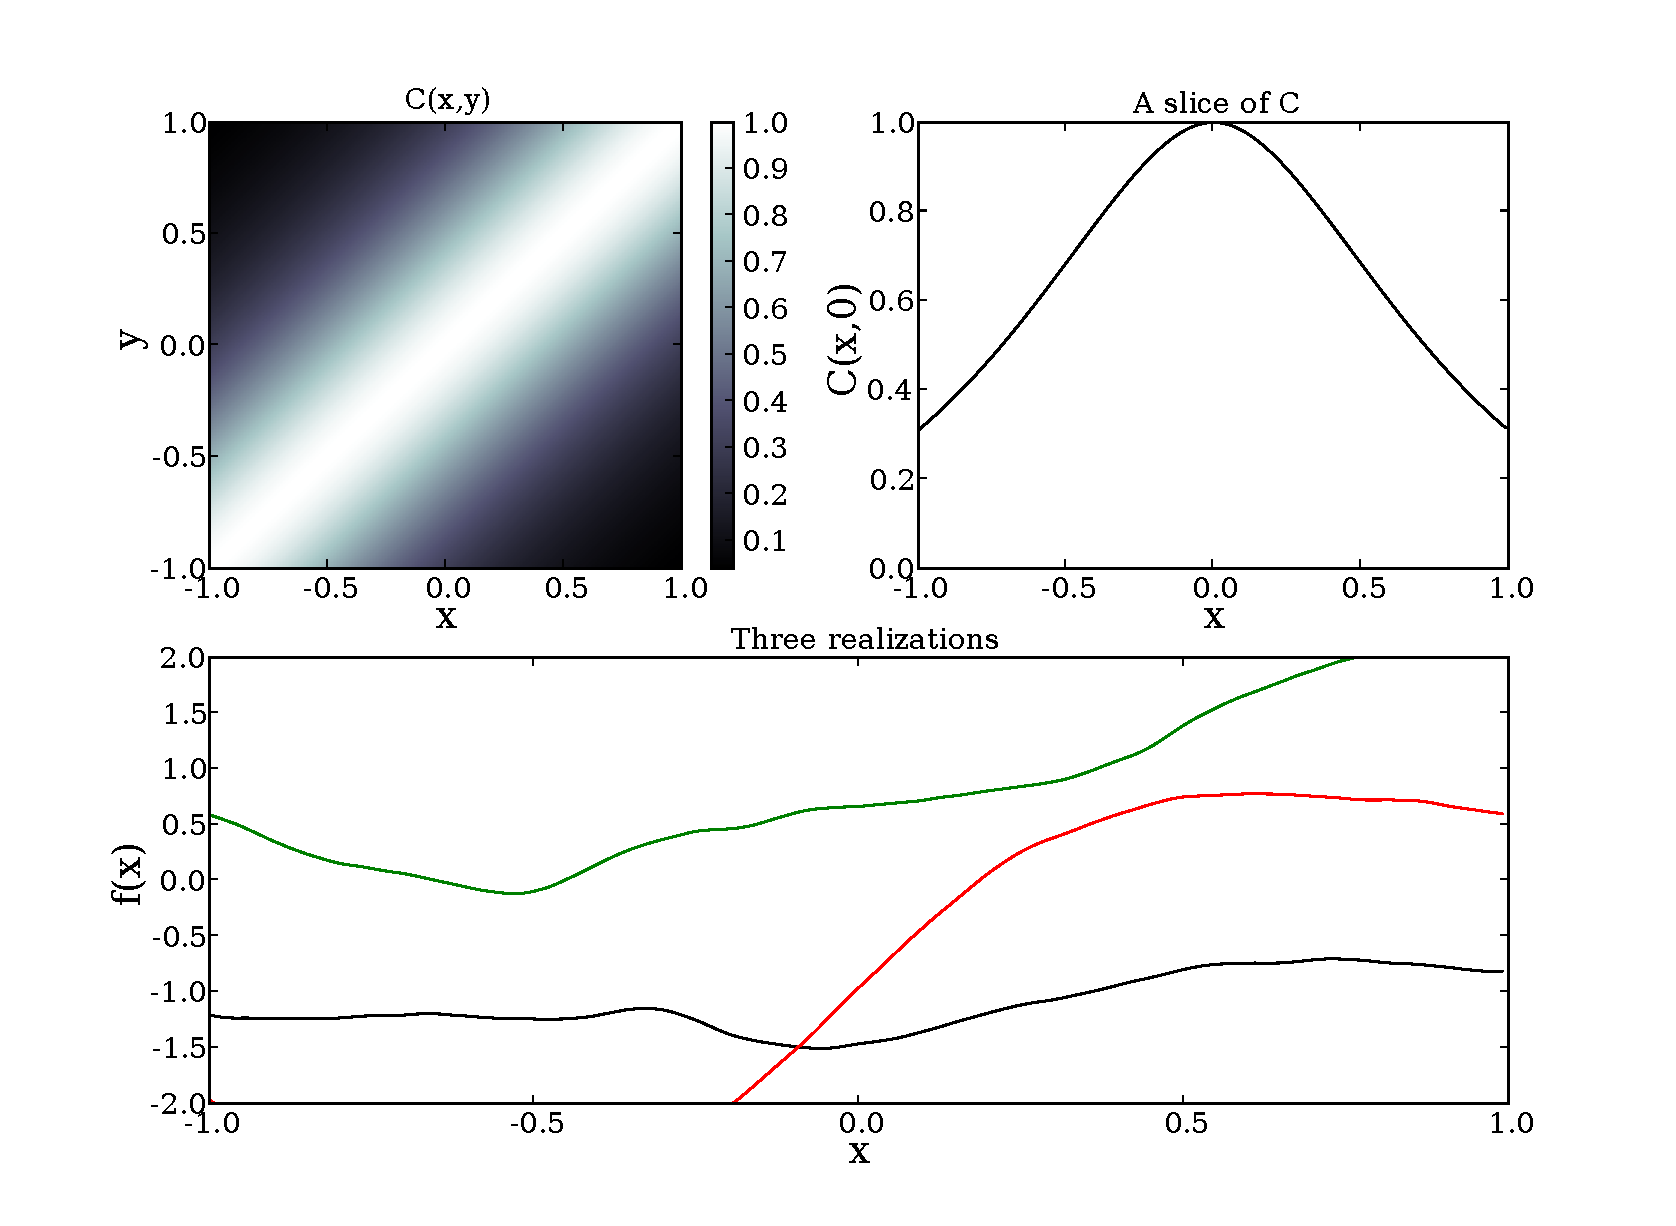
\epsfig{file=figs/d20a1s1.pdf,width=8cm}
        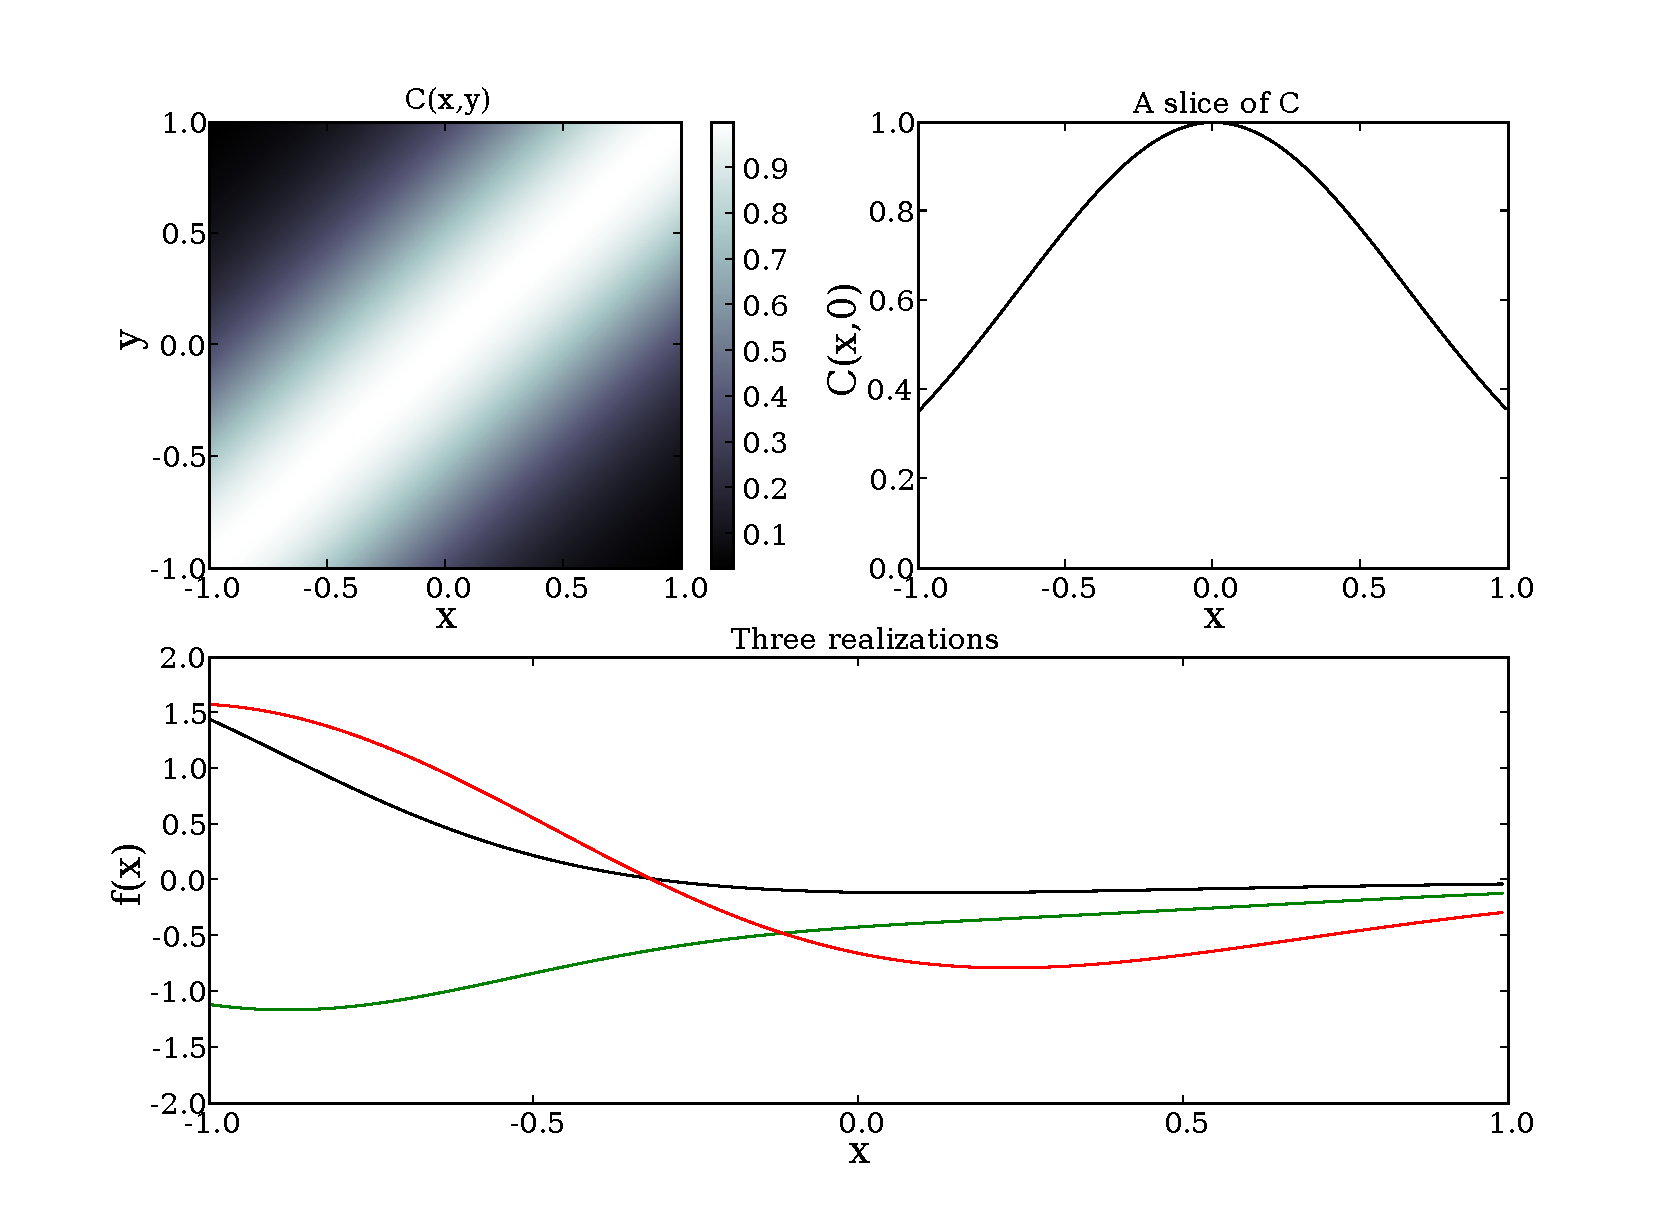
\epsfig{file=figs/d100a1s1.pdf,width=8cm}
    \caption{Matern draws for various \texttt{diff_degree} parameters. In increasing orders of smoothness: \texttt{.2}, \texttt{.5}, (equivalent to \texttt{pow_exp} with \texttt{pow=1}, roughness similar to Brownian motion), \texttt{1}, \texttt{1.4} (the examples given so far), \texttt{2}, \texttt{10} (nearly equivalent to \texttt{gaussian}).}
    \label{fig:diffdegree}
\end{figure}

\subsection{Suggestions for further experimentation}
\label{sec:experiment}


\begin{itemize}
    \item Change the parameters of the Mat\`ern covariance function, and try to guess how realizations will look.
    \item Differentiate realizations numerically. Recall that
    \begin{eqnarray*}
        \frac{df}{dx}=\lim_{h\rightarrow 0} \frac{f(x+h)-f(x)}{h},
    \end{eqnarray*}
    so you can take an approximate `numerical derivative' by evaluating the fraction on the right hand side with $h$ equal to a small number.
    \item Replace \texttt{matern.euclidean} in \file{examples/cov_params.py} with the Euclidean version of one of the other covariance functions and experiment with the parameters. See Banerjee \cite{banerjee} for their interesting properties.
    \item Replace \function{zero_fun} in \file{cov_params.py} with a nontrivial mean function and repeat the preceding.
\end{itemize}

\section{Nonparametric regression: observing Gaussian processes}\label{sec:observing}

\begin{figure}
    \centering
        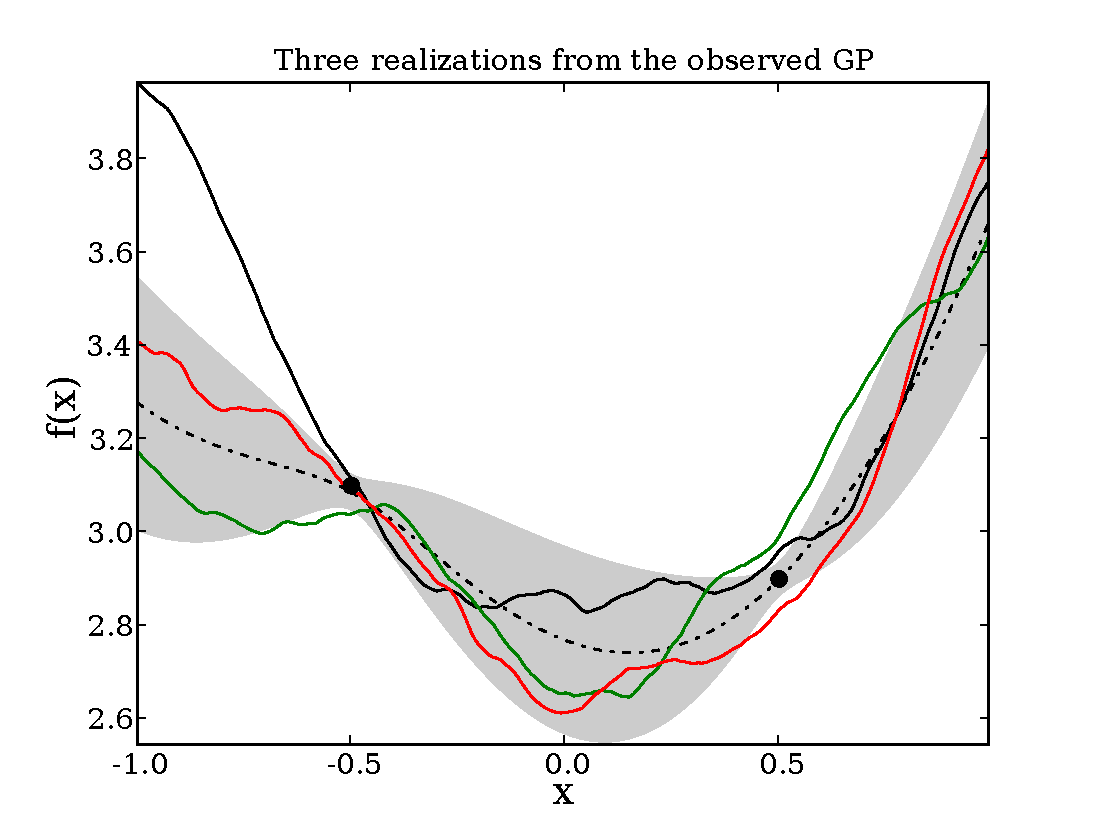
\epsfig{file=figs/obs.pdf,width=8cm}
        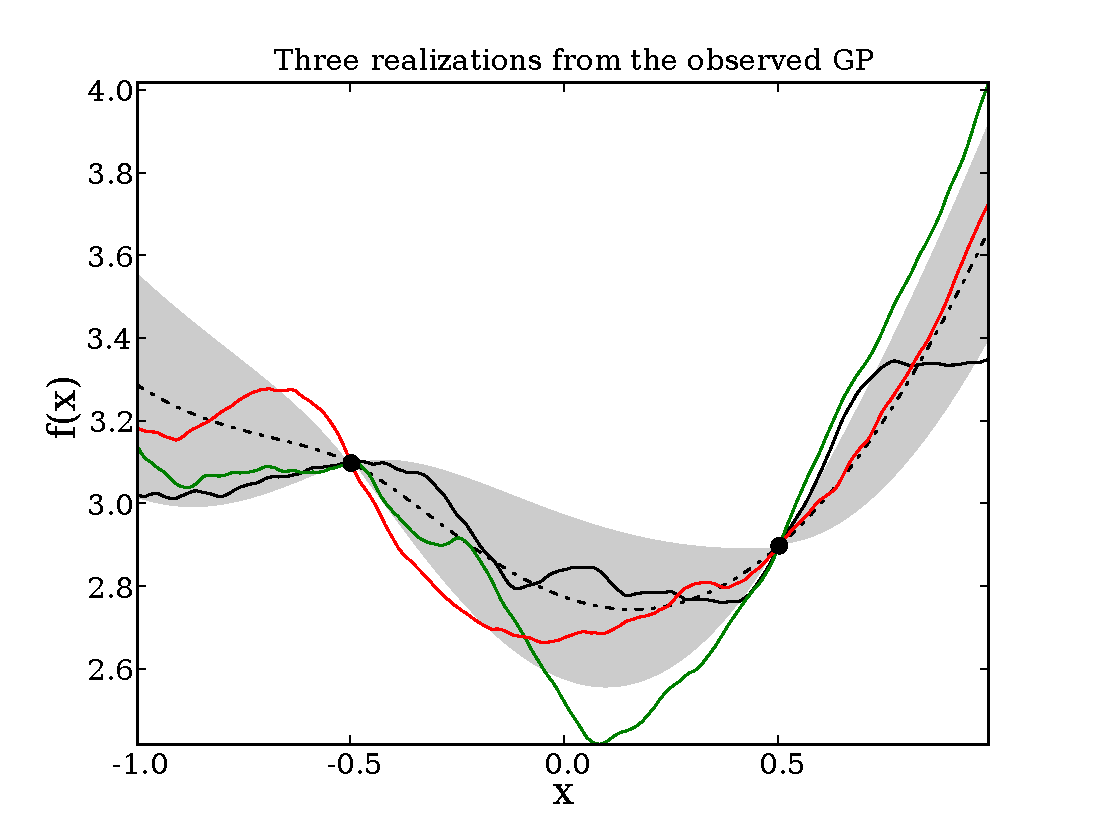
\epsfig{file=figs/cond.pdf,width=8cm}
    \caption{The output of {\sffamily `examples/observations.py'}: the observed GP with \texttt{obs_V = .002} (left) and \texttt{obs_V = 0} (right). Note that in the conditioned case, the $\pm$ 1 SD envelope shrinks to zero at the points where the observations were made, and all realizations pass through the observed values. Compare these plots to those in figure \ref{fig:realizations}.}
    \label{fig:obs}
\end{figure}

Consider the following common statistical situation: You decide on a GP prior for an unknown function $f$, then you observe the value of $f$ at $N$ input points $[o_0\ldots o_{N-1}]$, possibly with uncertainty. If the observation error is normally distributed, it turns out that $f$'s posterior distribution given the new information is another Gaussian process, with new mean and covariance functions.

The probability model that represents this situation is as follows:
\begin{equation}
    \label{regprior}
    \left.\begin{array}{l}
        \textup{data}_i \stackrel{\tiny{\textup{ind}}}{\sim} \textup{N}(f(o_i), V_i)\\
        f \sim \textup{GP}(M,C)\\
    \end{array}\right\}\Rightarrow f|\textup{data} \sim \textup{GP}(M_o, C_o).
\end{equation}
This package provides a function called \function{observe} that imposes normally-distributed observations on Gaussian process distributions. This function converts $f$'s prior to its posterior by transforming $M$ and $C$ in equation \ref{regprior} to $M_o$ and $C_o$:

The following code (from \file{observation.py}) imposes the observations
\begin{eqnarray*}
    f(-.5) = 3.1\\
    f(.5) = 2.9
\end{eqnarray*}
with observation variance $V=.002$ on the GP distribution defined in \file{mean.py} and \file{cov.py}:
\verbatiminput{../../examples/gp/observation.py}

The function \function{observe} takes a covariance $C$ and a mean $M$ as arguments, and essentially tells them that their realizations' values on \code{obs_mesh} have been observed to be \code{obs_vals} with variance \code{obs_V}. If \code{obs_V} is \code{None}, \function{observe} assumes that the observation precision was infinite; that is, that the realizations' values on \code{obs_mesh} were observed with no uncertainty. Making (or pretending to make) observations with infinite precision is sometimes called \emph{conditioning}, and can be a valuable tool for modifying GP priors; for example, if a rate function is known to be zero when a population's size is zero.

The output of the code is shown in figure \ref{fig:obs}, along with the output with \code{obs_V=None}. Compare these to the analogous figure for the unobserved GP, figure \ref{fig:realizations}. The covariance after observation is visualized in figure \ref{fig:obscov}. The covariance `tent' has been pressed down at points where $x\approx \pm .5$ and/or $y\approx\pm .5$, which are the values where the observations were made.

\begin{figure}
    \centering
        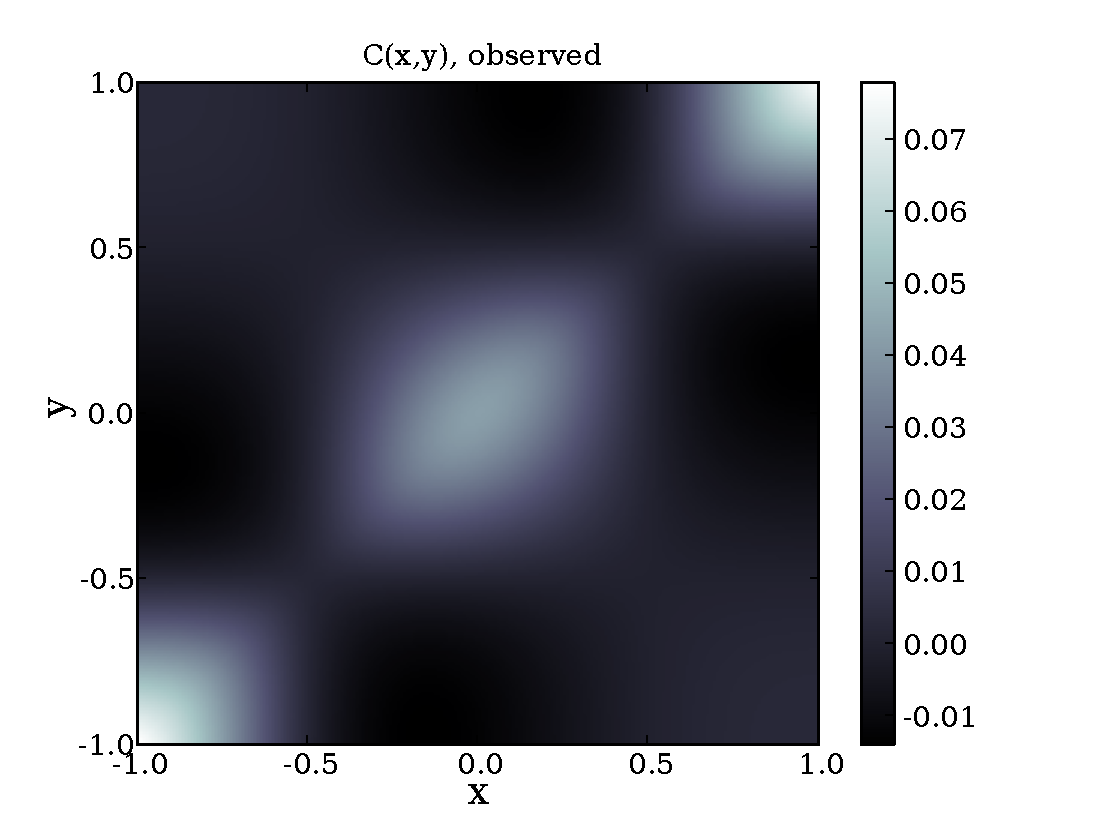
\epsfig{file=figs/obscov.pdf,width=10cm}
    \caption{The covariance function from {\sffamily `observation.py'} after observation. Compare this with the covariance function before observation, visualized in figure \ref{fig:cov} }
    \label{fig:obscov}
\end{figure}

\subsection{Example: Salmonid stock-recruitment functions}\label{sub:MMKregression}
Munch, Kottas and Mangel \cite{mmk} use Gaussian process priors to infer various \emph{stock-recruitment (SR) functions}. An important concept in fishery science, SR functions relate the size of a fish stock to the number or biomass of recruits to the fishery each year. In other words, they relate population size or biomass to number or biomass of new fish produced. The authors argue that model uncertainty is endemic in stock-recruitment theory, and that in this situation GP priors are a sensible alternative to particular functional forms.

We don't have the tools yet to fully duplicate Munch, Kottas and Mangel' results; that will have to wait for chapter \ref{cha:PyMC}. However, we can fit a simpler version of their model now by using the \function{observe} function. Specifically, we'll fit the data in figure 6 of their paper \cite{mmk}, which is for three salmonids: chum (\emph{Onchorhynchus keta}), pink (\emph{Onchorhynchus gorbuscha}) and sockeye (\emph{Onchorhynchus nerka}).

The code is in the script \file{examples/gp/more_examples/MMKsalmon/regression.py}. The script begins by importing the \class{salmon} class from \file{salmon.py} in the same directory.
The \class{salmon} class does the following:
\begin{itemize}
    \item Reads data from a csv file.
    \item Creates a GP prior with a Mat\`ern covariance function and a linear mean function. The parameters are chosen fairly arbitrarily at this stage. In chapter \ref{cha:PyMC}, we'll look at how to place priors on these parameters and infer them along with the unknown function itself.

    Note also that I've specified the prior using the data; for instance, the \texttt{scale} parameter depends on the maximum observed abundance. Some would consider this cheating.
    \item `Observes' the unknown function's value to be zero at the origin with no uncertainty. No matter what the data are, every draw from the posterior will have $f(0) = 0$. This isn't really an observation, it's just a convenient way to incorporate the knowledge that if there is no stock, there will be no recruitment.
    \item Provides a \method{plot} method, which just plots the posterior envelope, data and three realizations from the posterior.
\end{itemize}
% The code in \file{examples/more_examples/MKMsalmon/salmon.py} is shown here:
% \verbatiminput{../../examples/gp/more_examples/MKMsalmon/salmon.py}

\begin{figure}
    \centering
        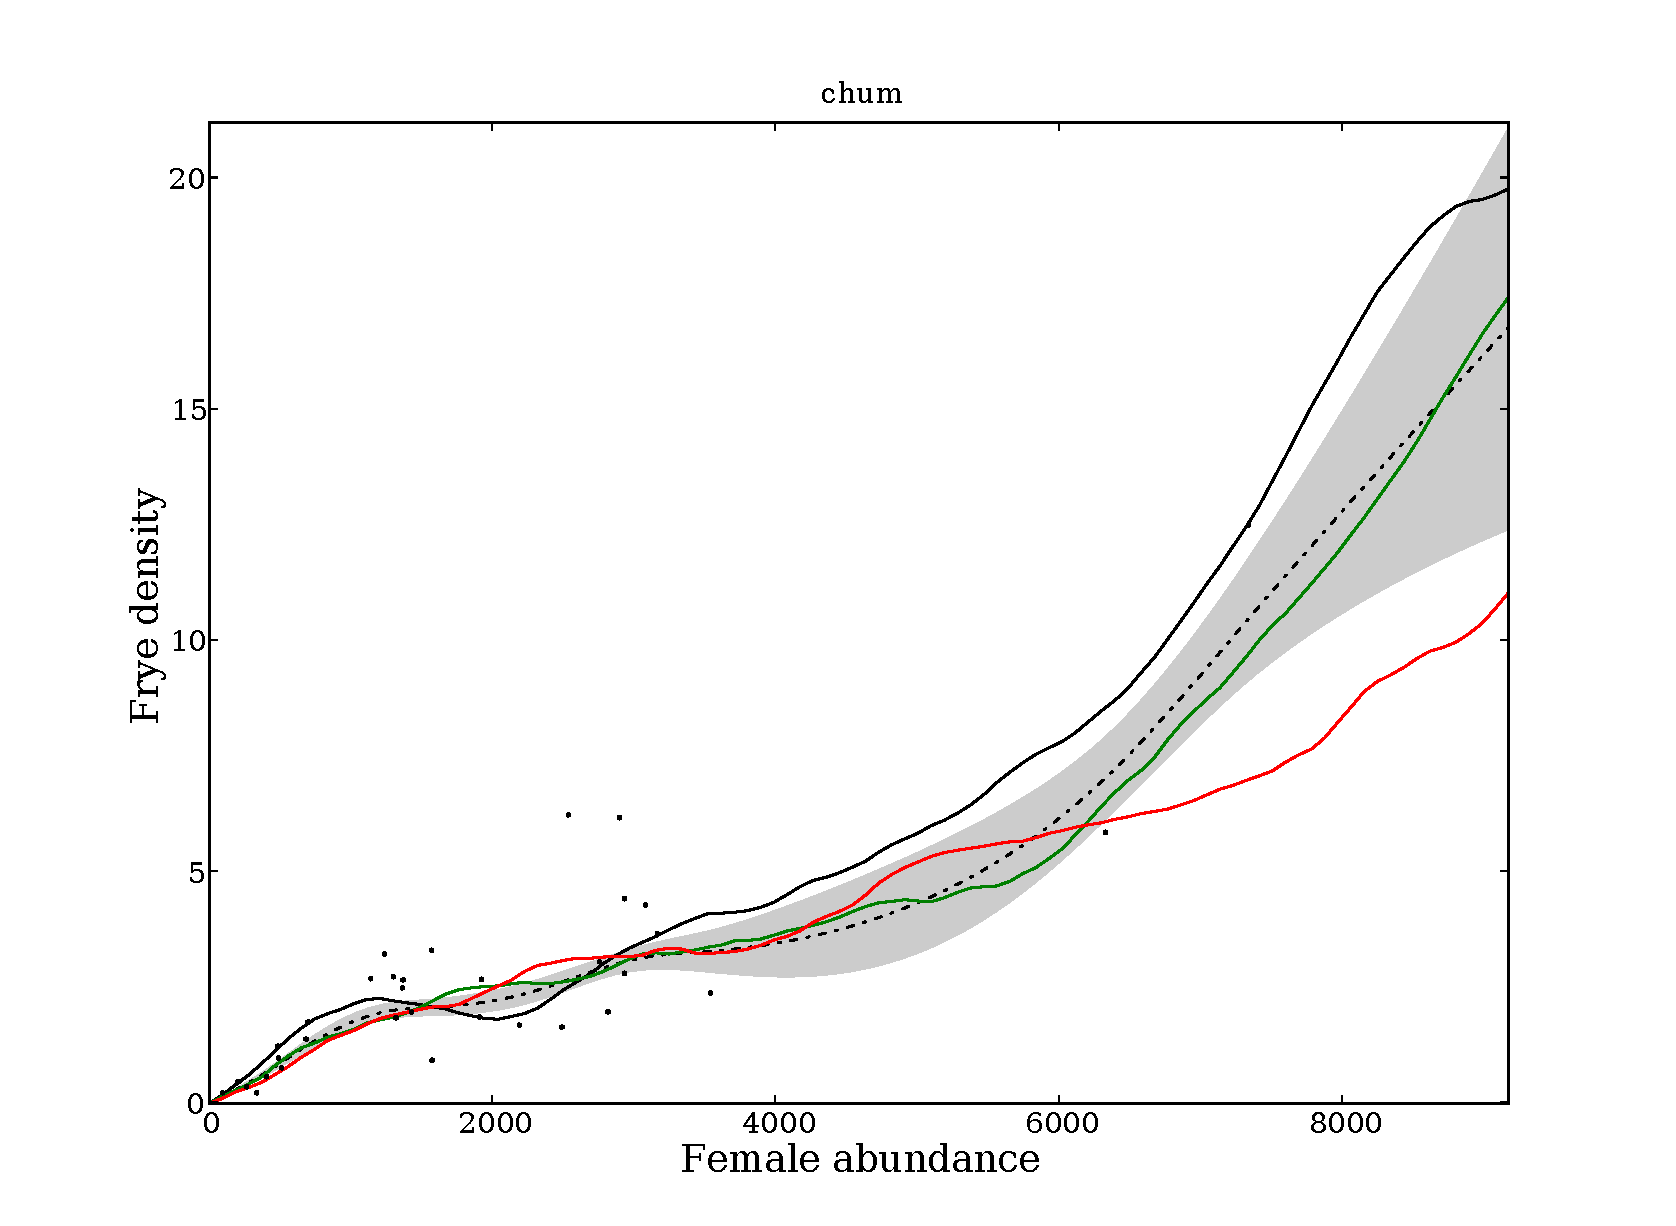
\epsfig{file=figs/MMKchumreg.pdf,width=10cm}
        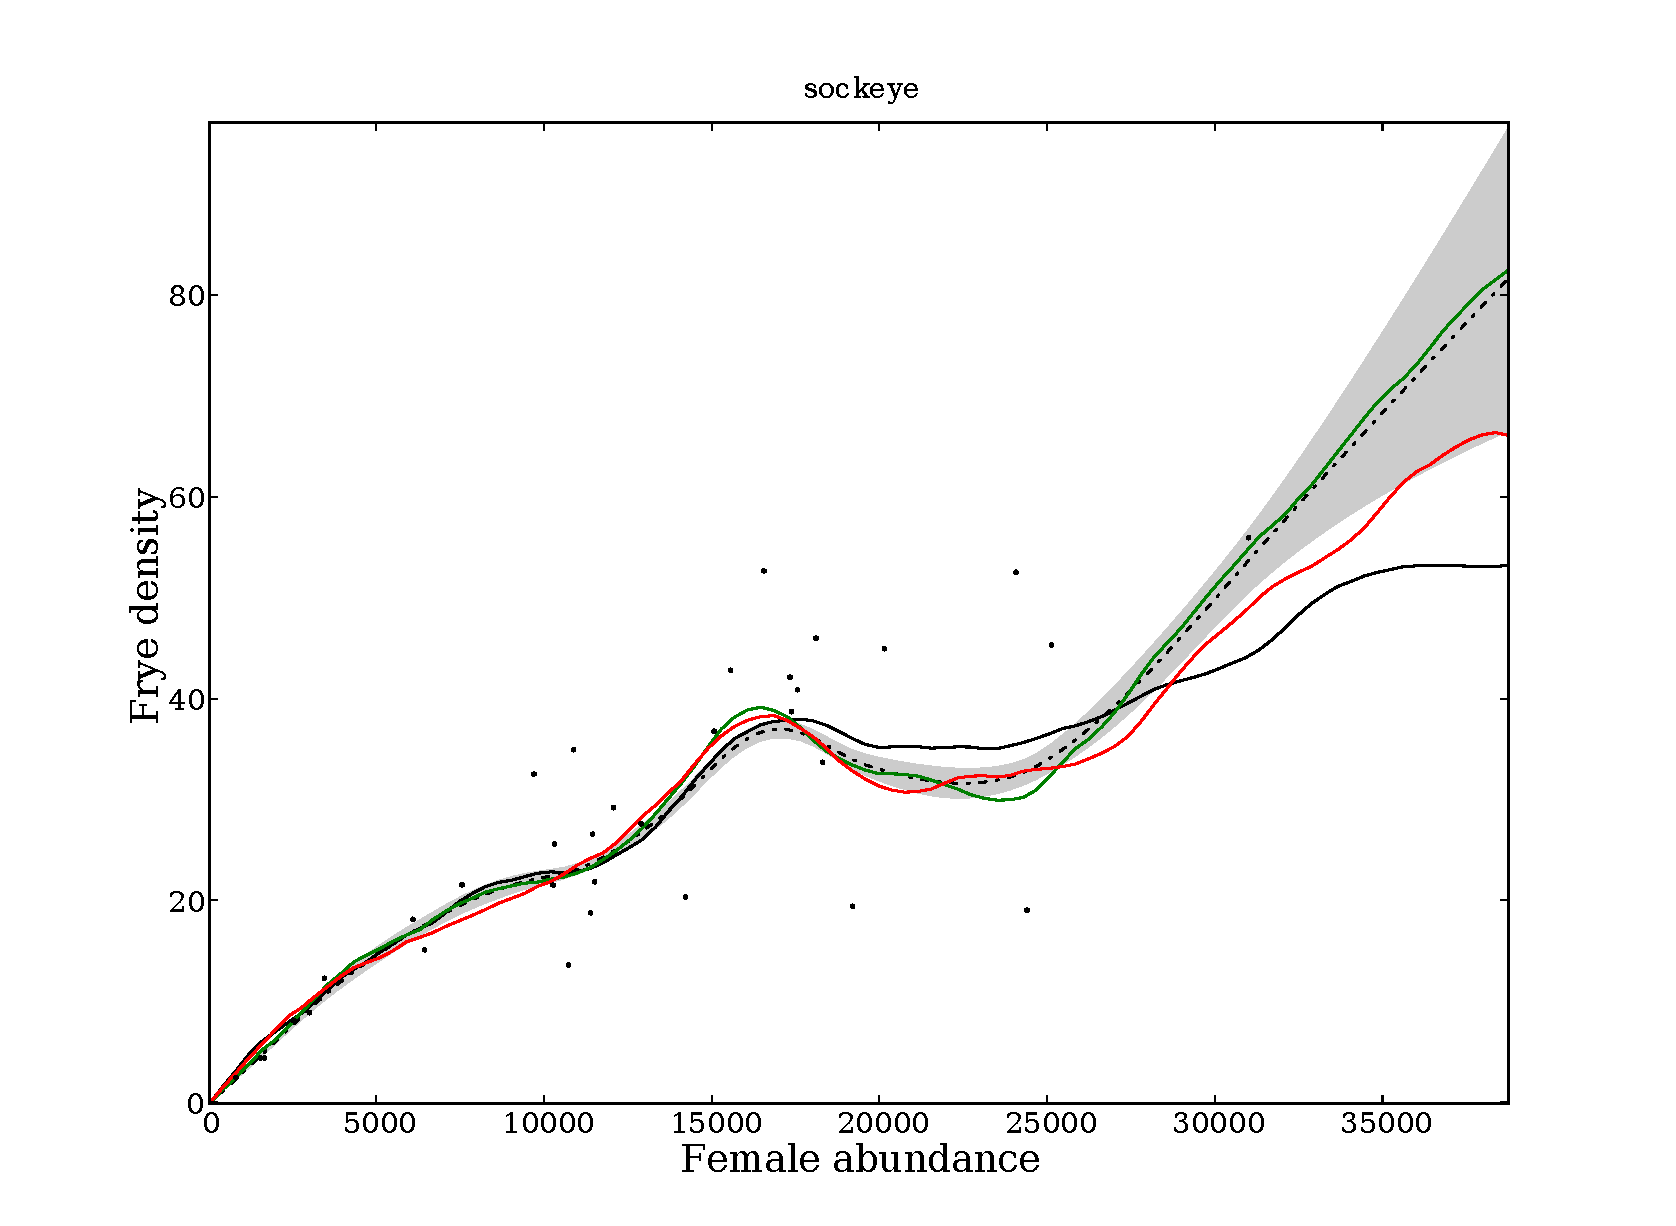
\epsfig{file=figs/MMKsockeyereg.pdf,width=10cm}
        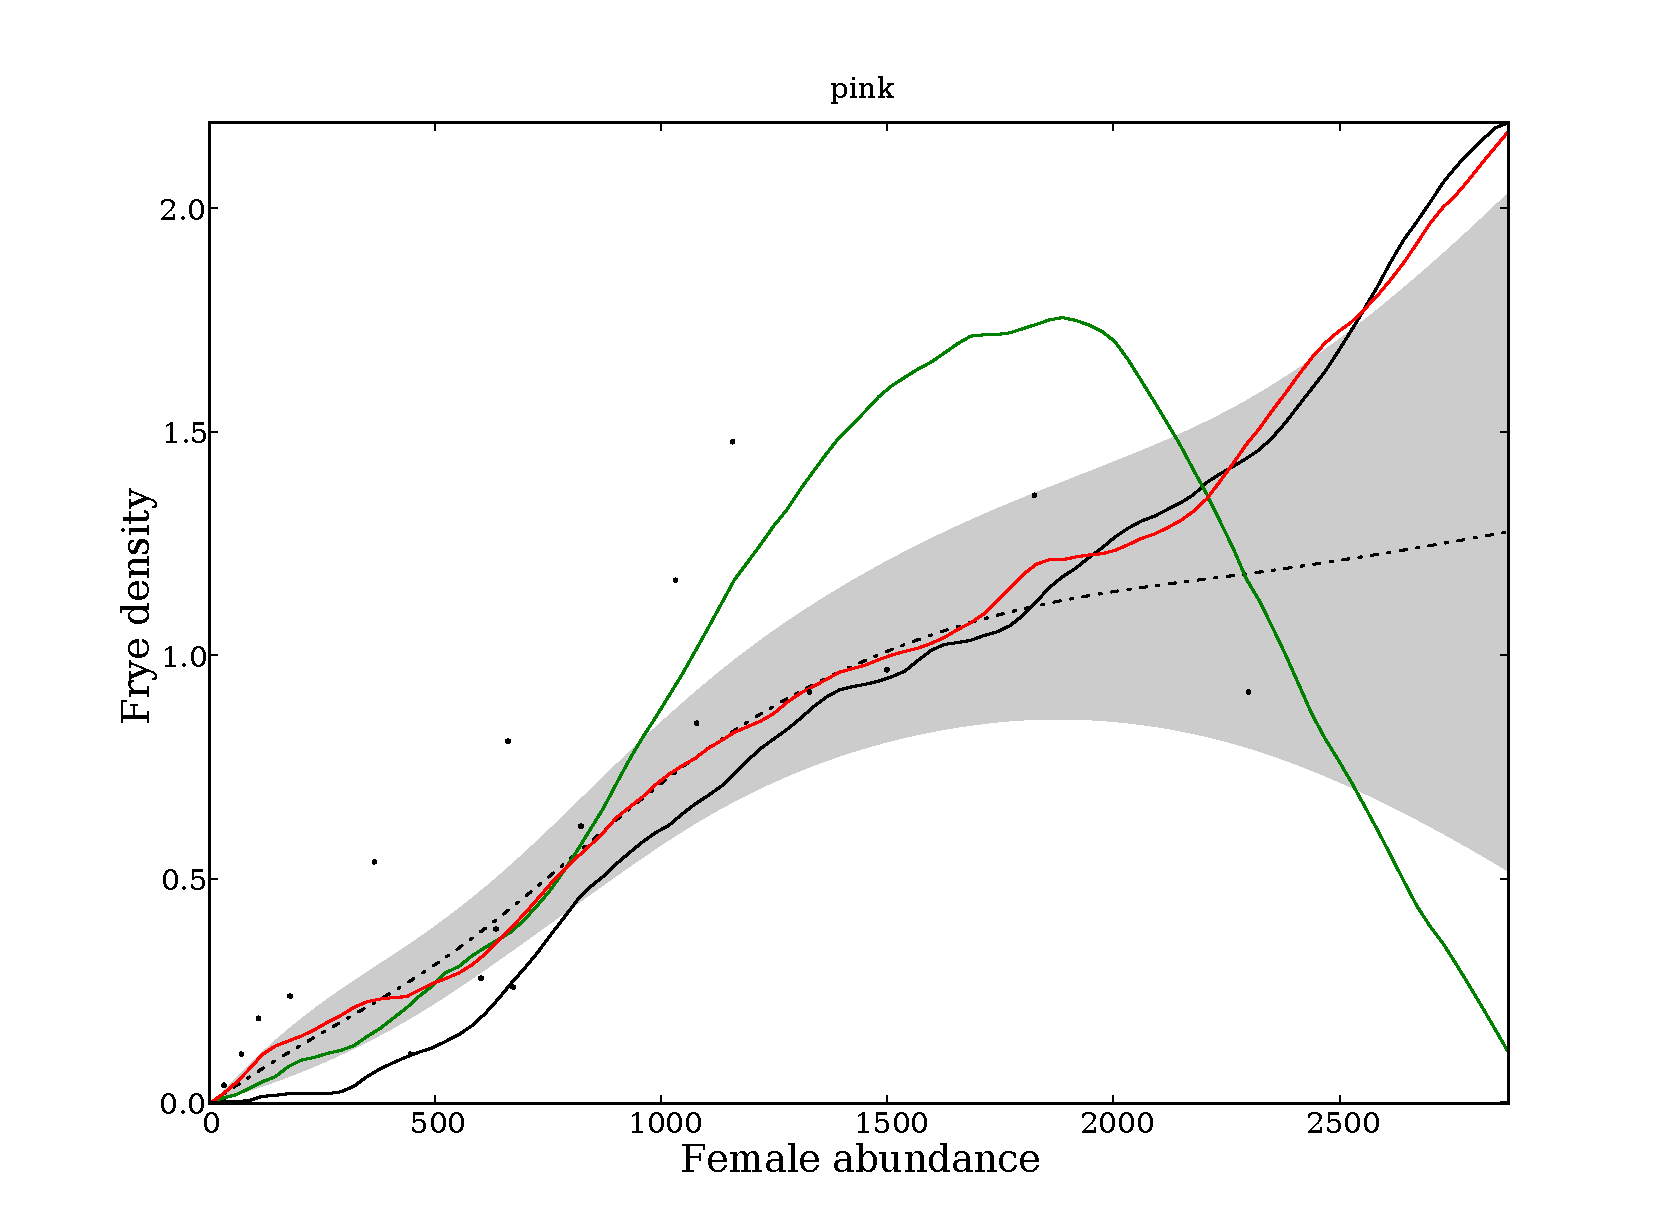
\epsfig{file=figs/MMKpinkreg.pdf,width=10cm}
    \caption{Fits to the stock-recruitment data in Munch, Kottas and Mangel' \cite{mmk} Figure 6 using a simple nonparametric regression.}
    \label{fig:MMKregression}
\end{figure}

The main script, \file{examples/more_examples/MKMsalmon/salmon.py}, creates three \class{salmon} instances called \texttt{chum}, \texttt{pink} and \texttt{sockeye}, then imposes the data for each species on its prior to obtain its posterior. The observation variance I used was chosen fairly arbitrarily like the prior parameters, and we'll look at inferring it in chapter \ref{cha:PyMC} also. Finally, each species' \method{plot} method is called. Output is shown in figure \ref{fig:MMKregression}.
% The code in \file{examples/more_examples/MKMsalmon/regression.py} is shown here:
% \verbatiminput{../../examples/gp/more_examples/MKMsalmon/regression.py}

To reiterate, there are some major drawbacks to this simple model. The observation variance may not actually be known, and we may not be comfortable specifying a single value for each of the prior parameters. Because of these considerations, Munch, Kottas and Mangel opt for a more sophisticated statistical model that has to be fit using MCMC. We will follow them in section \ref{sub:MMKMCMC}.

\section{Higher-dimensional GPs}\label{sec:highdim}

In addition to functions of one variable such as $f(x)$, this package supports Gaussian process priors for functions of many variables such as $f(\mathbf{x})$, where $\mathbf{x}=[x_0\ldots x_{n-1}]$. This is useful for modeling dynamical or biological functions of many variables as well as for spatial statistics.

Any time you pass an array into a \texttt{Mean}, \texttt{Covariance} or \texttt{Realization}'s init method or evaluate one of these objects on an array, the convention is that the array's last index iterates over spatial dimension. To evaluate a covariance C on the ordered pairs \texttt{(0,1)}, \texttt{(2,3)}, \texttt{(4,5)} and \texttt{(6,7)}, you could pass in the following two-dimensional array:
\begin{verbatim}
[[0,1]
 [2,3]
 [4,5]
 [6,7]]
\end{verbatim}
or the following three-dimensional array:
\begin{verbatim}
[[[0,1]
  [2,3]],

  [4,5]
  [6,7]]]
\end{verbatim}
Either is fine, since in both the last index iterates over elements of the ordered pairs.

The exception to this rule is one-dimensional input arrays. The array
\begin{verbatim}
[0, 1, 2, 3, 4, 5, 6, 7]
\end{verbatim}
is interpreted as an array of eight one-dimensional values, whereas the array
\begin{verbatim}
[[0, 1, 2, 3, 4, 5, 6, 7]]
\end{verbatim}
is interpreted as a single eight-dimensional value according to the convention above.

Means and covariances learn their spatial dimension the first time they are called or observed. Some covariances, such as those specified in geographic coordinates, have an intrinsic spatial dimension. Realizations inherit their spatial dimension from their means and covariances when possible, otherwise they learn it the first time they are called. If one of these objects is subsequently called with an input of a different dimension, it raises an error.

\subsection{Covariance function bundles and coordinate systems}
The examples so far, starting with \file{examples/cov.py}, have used the covariance function \texttt{matern.euclidean}. This function is an attribute of the \texttt{matern} object, which is an instance of class \class{covariance_function_bundle}.

Instances of \class{covariance_function_bundle} have three attributes, \texttt{euclidean}, \texttt{geo_deg} and \texttt{geo_rad}, which correspond to standard coordinate systems:
\begin{itemize}
    \item \texttt{euclidean}: $n$-dimensional Euclidean coordinates.
    \item \texttt{geo_deg}: Geographic coordinates (longitude, latitude) in degrees, with radius 1.
    \item \texttt{geo_rad}: Geographic coordinates (longitude, latitude) in radians, with radius 1.
\end{itemize}
Note that you can effectively change the radius of the geographic coordinate systems using the \texttt{scale} parameter.

Covariance function bundles are described in more detail in section \ref{cha:usercov}.

\subsection{Multithreading GP operations}
This package can use multi-core systems to speed up two kinds of computations:
\begin{itemize}
	\item filling in covariance matrices,
	\item linear algebra for observing GP's or drawing realizations.
\end{itemize}
If you've built NumPy against multithreaded linear algebra libraries, all the linear algebra will be parallelized automatically. The functions contained in covariance function bundles (section \ref{cha:usercov}), which include all the covariance functions distributed with this package, are multithreaded. The number of threads they use is controlled by the environment variable \code{OMP_NUM_THREADS}. 

On a quad-core system, evaluating a covariance function on large input vectors when \texttt{OMP_NUM_THREADS} is equal to 4 will use all the cores. Note that there's no point setting \texttt{OMP_TUM_THREADS} to 5 on a quad-core system, because only four cores are available.


\subsection{A geostatistical example}\label{sub:geostat}
\begin{figure}
    \centering
        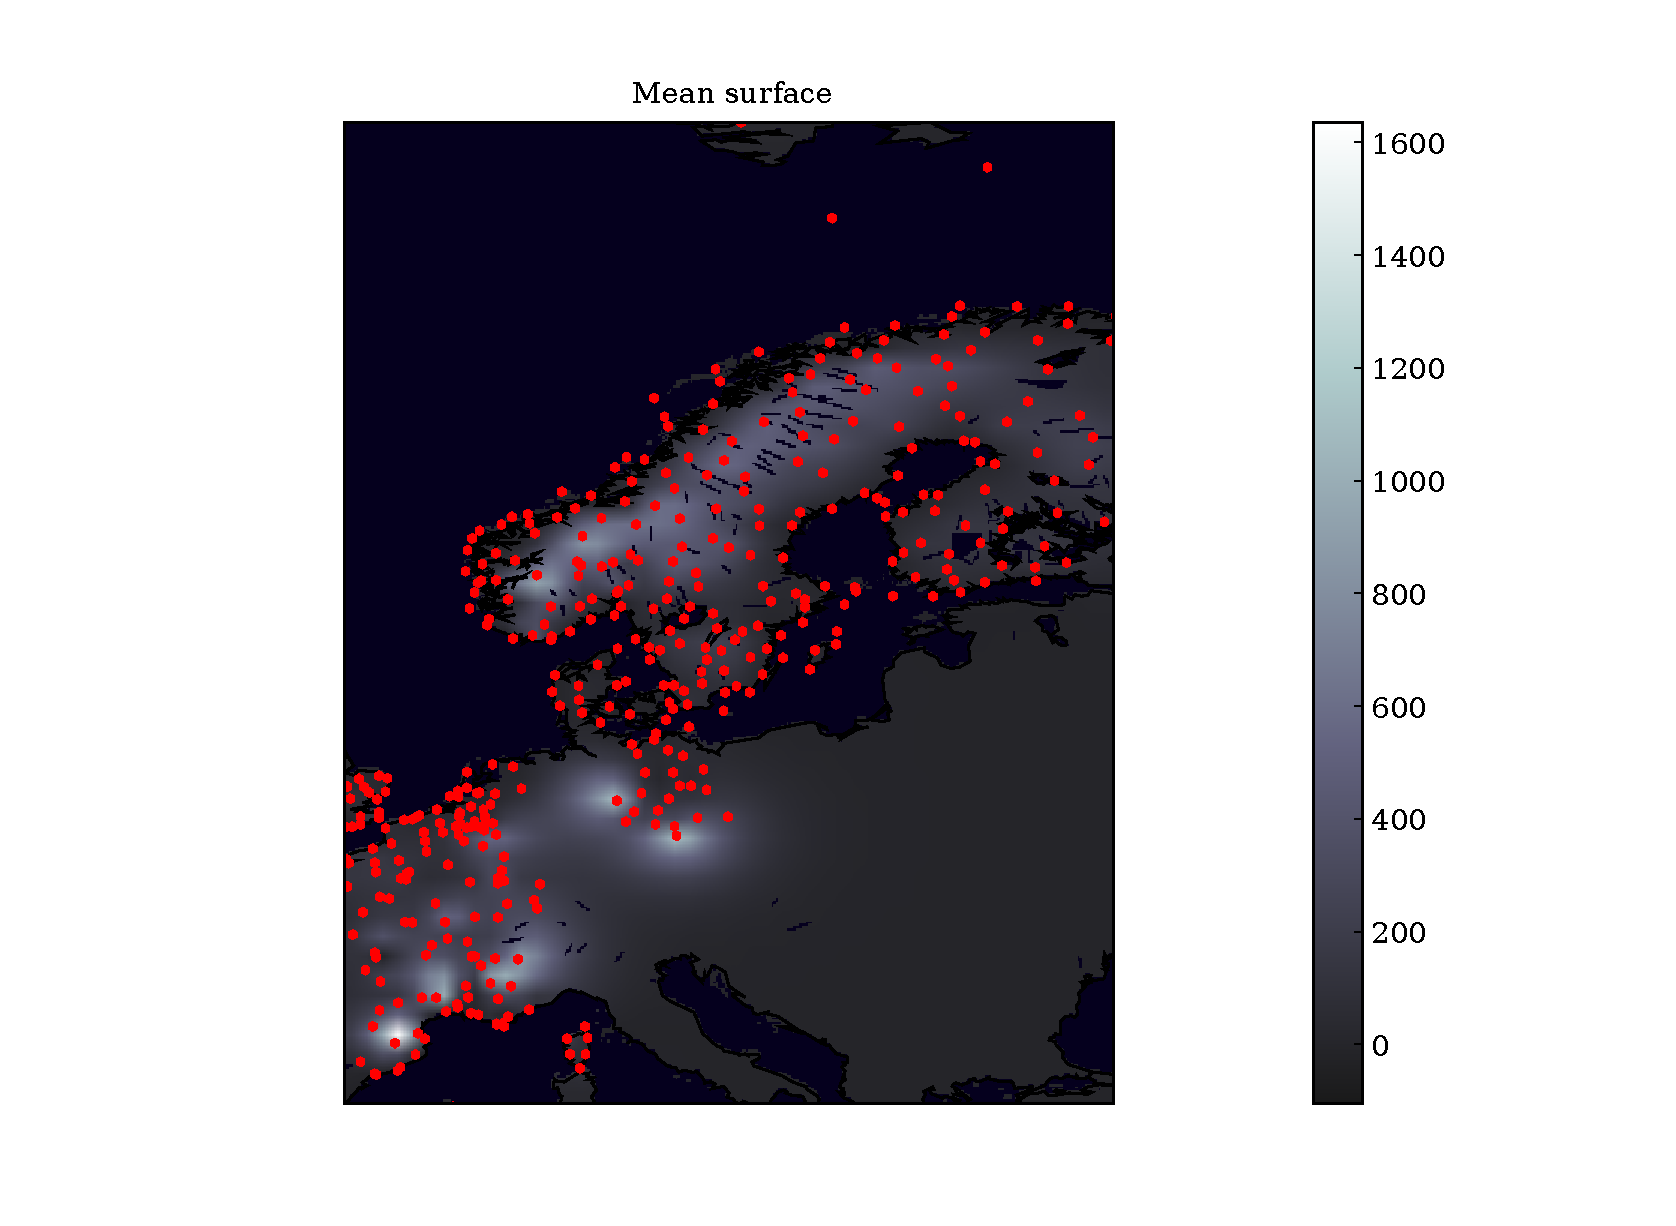
\epsfig{file=figs/elevmean.pdf, width=8cm}
        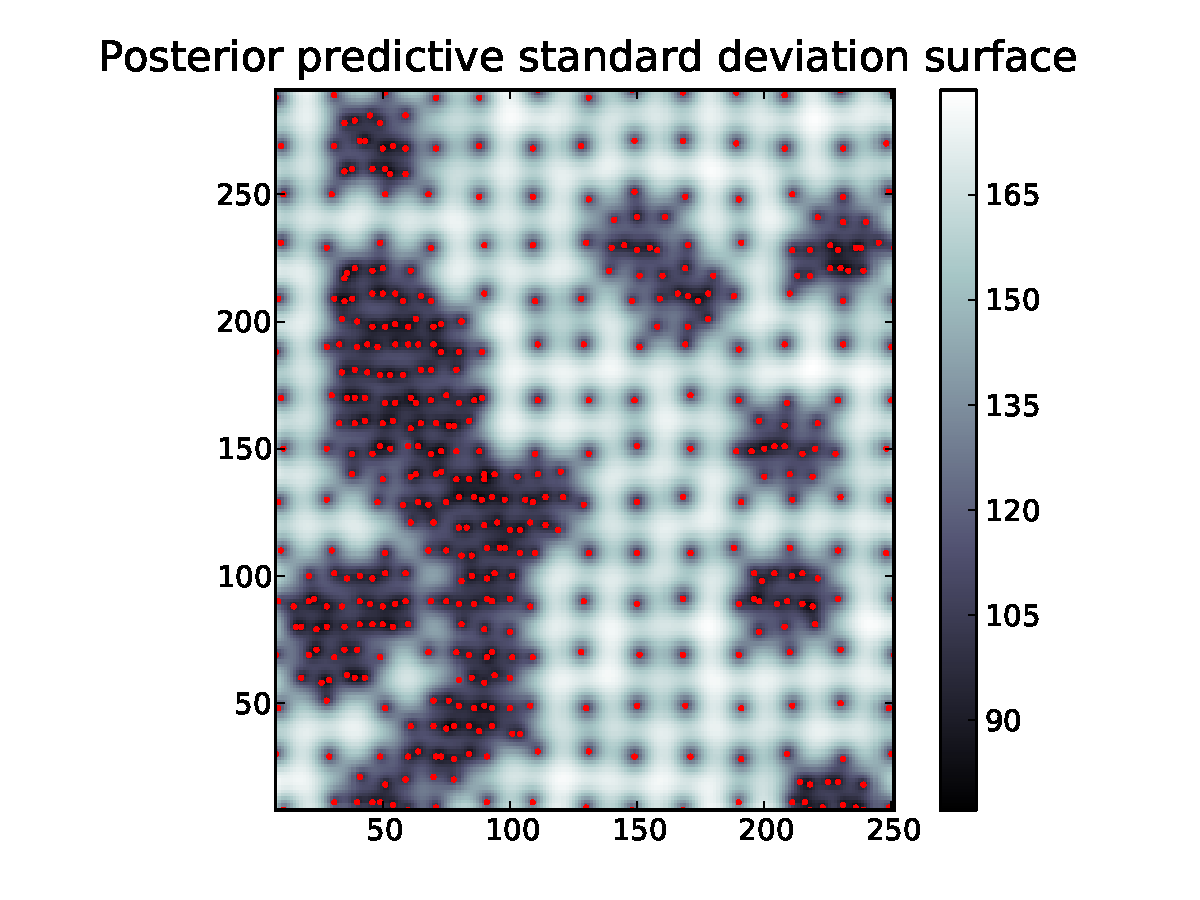
\epsfig{file=figs/elevvar.pdf, width=8cm}
    \caption{The posterior mean and variance surfaces for the elevation example. Elevation is measured in meters. Computing these surfaces is also called `\citetitle[http://en.wikipedia.org/wiki/Kriging]{simple kriging}.' The posterior variance is small in the neighborhood of observations, but large in regions where no observations were made. Note that this posterior distribution is conditional on a relatively sparse dataset, which notably misses some of the highest points in Europe.}
    \label{fig:elev}
\end{figure}
\begin{figure}
    \centering
        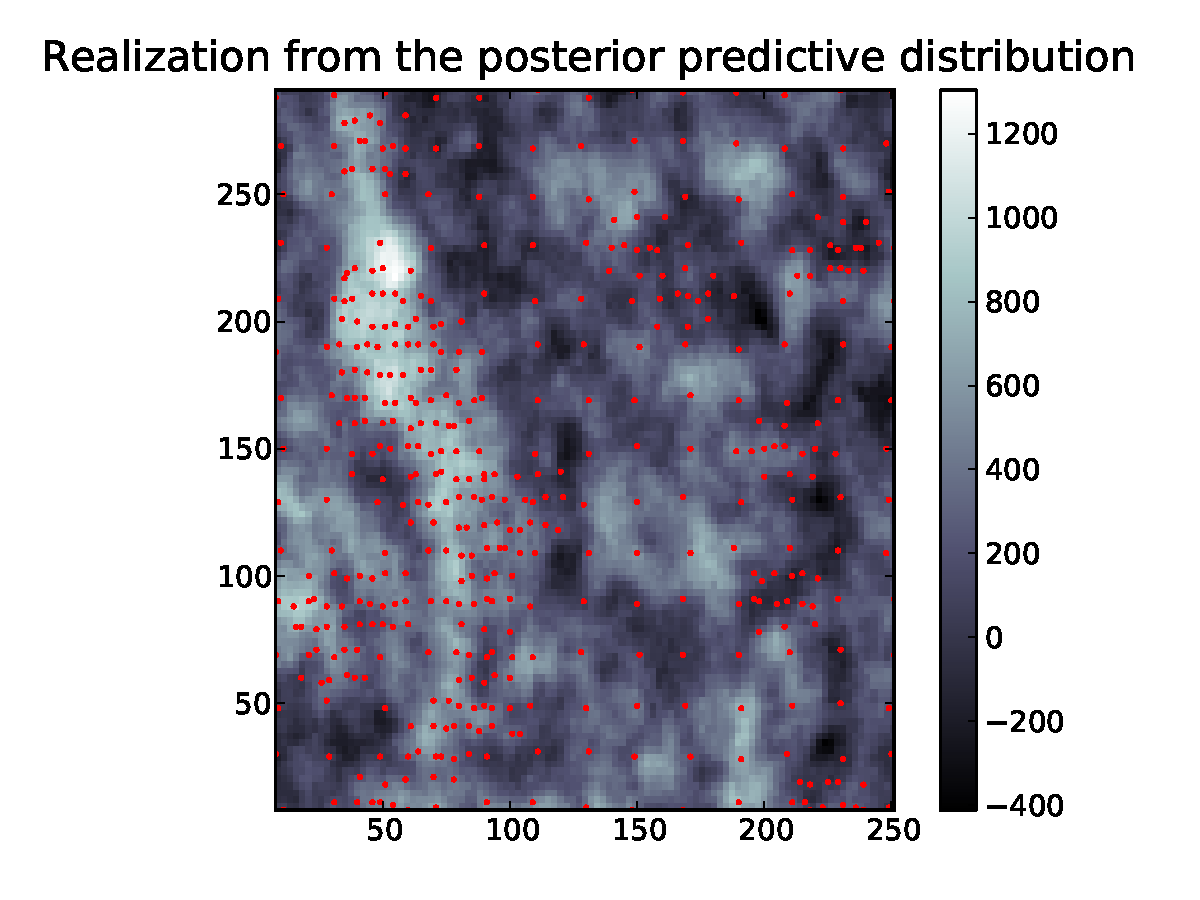
\epsfig{file=figs/elevdraw0.pdf, width=8cm}
        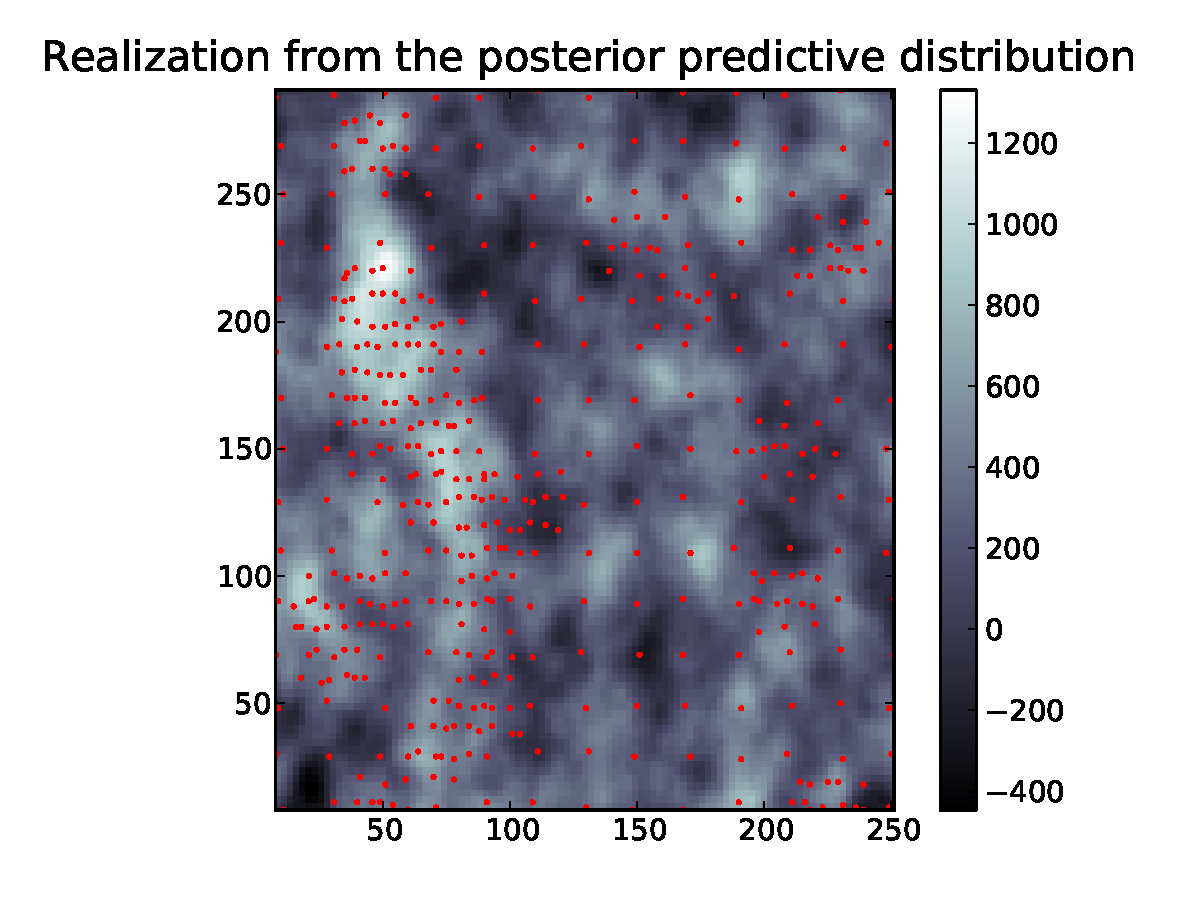
\epsfig{file=figs/elevdraw1.pdf, width=8cm}
    \caption{Two realizations from the posterior distribution of elevation. Elevation is measured in meters.}
    \label{fig:elevreal}
\end{figure}
Higher-dimensional usage is demonstrated in the folder \file{examples/gp/more_examples/Elevation}. File \file{getdata.py} extracts latitude, longitude and elevation data from the csv file in that folder and manipulates them into the array format described in section \ref{sec:highdim}. The data are from the Carbon Dioxide Information Analysis Center's \citetitle[http://cdiac.ornl.gov/epubs/ndp/ndp026d/ndp026d.html]{Cloud Climatology for Land Stations Worldwide, 1971-1996}. File \file{makemap.py} interfaces with \citetitle[www.matplotlib.org]{matplotlib}'s \texttt{basemap} toolkit, which draws maps. File \file{regression.py} actually implements the regression.
% \verbatiminput{../../examples/gp/more_examples/Elevation/regression.py}

The output of \file{regression.py} is shown in figures \ref{fig:elev} and \ref{fig:elevreal}. Figure \ref{fig:elev} shows the posterior mean and variance of the elevation. Finding these surfaces is also known as `\citetitle[http://en.wikipedia.org/wiki/Kriging]{simple kriging}.' Note that it's not possible to visualize the full covariance matrix, because it's now a function of four variables. The surface in figure \ref{fig:elev} is equivalent to the diagonal of the surface in figure \ref{fig:obs}.

Figure \ref{fig:elevreal} shows two realizations from the posterior distribution of the elevation surface. They are much rougher than their mean surface. Evaluating realizations is much more expensive than evaluating the observed mean or evaluating the observed covariance with one argument.


\section{Basis covariances}\label{sec:basis}

\begin{figure}[htbp]
    \centering
        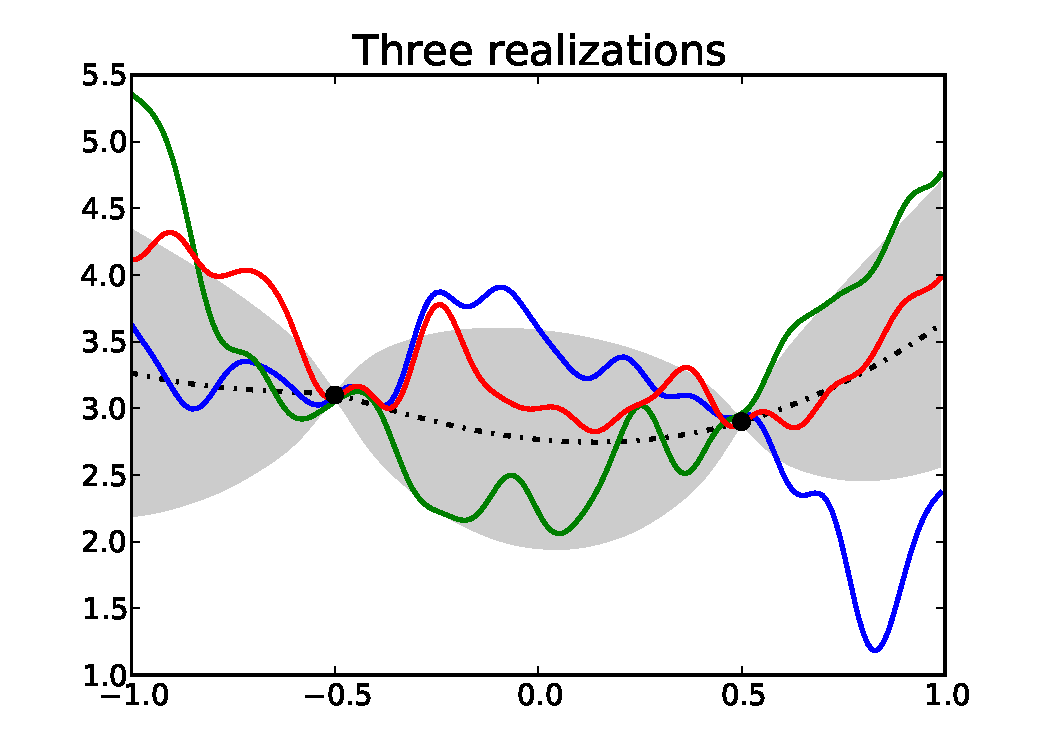
\epsfig{file=figs/basiscov.pdf,width=10cm}
        \caption{Three realizations of an observed Gaussian process whose covariance is an instance of \class{BasisCovariance}. The basis in this case is function \function{fourier_basis} from module \module{cov_funs}. 25 basis functions are used.}
    \label{fig:basiscov}
\end{figure}

It's possible to create random functions from linear combinations of finite sets of basis functions $\{e\}$ with random coefficients $\{c\}$:
\begin{eqnarray*}
    f(x) = M(x) + \sum_{i_0=0}^{n_0-1}\ldots \sum_{i_{N-1}=0}^{n_{N-1}-1} c_{i_1\ldots i_{N-1}} e_{i_1\ldots i_{N-1}}(x), &
    \{c\}\sim \textup{some distribution}.
\end{eqnarray*}
If the distribution is multivariate normal with mean zero, $f$ is a Gaussian process with mean $M$ and covariance defined by
\begin{eqnarray*}
    C(x,y)=\sum_{i_0=0}^{n_0-1}\ldots \sum_{i_{N-1}=0}^{n_{N-1}-1} \sum_{j_0=0}^{n_0-1}\ldots \sum_{j_{N-1}=0}^{n_{N-1}-1} e_{i_0\ldots i_{N-1}}(x) e_{j_1\ldots j_{N-1}}(x) K_{i_0\ldots i_{N-1}, j_1\ldots j_{N-1}},
\end{eqnarray*}
where $K$ is the covariance of the coefficients $c$.

Particularly successful applications of this general idea (shown in one dimension) are:
\begin{description}
    \item[Random Fourier series:] $e_i(x) = \sin(i\pi x/L)$ or $\cos(i\pi x/L)$, for instance \cite{spanos}.
    \item[Gaussian process convolutions:] $e_i(x) = \exp(-(x-\mu_n)^2)$, for instance \cite{convolution}.
    \item[B-splines:] $e_i(x) = $ a polynomial times an interval indicator. See \citetitle[http://en.wikipedia.org/wiki/Basis_B-spline]{Wikipedia}'s article.
\end{description}
Such representations can be very efficient when there are many observations in a low-dimensional space, but are relatively inflexible in that they generally produce realizations that are infinitely differentiable. In some applications, this tradeoff makes sense.

This package supports basis representations via the \class{BasisCovariance} class:
\begin{verbatim}
    C = BasisCovariance(basis, cov, **basis_params)
\end{verbatim}
The arguments are:
\begin{description}
    \item[\texttt{basis}:] Must be an array of functions, of any shape. Each basis function will be evaluated at \texttt{x} with the extra parameters. The basis functions should obey the same calling conventions as mean functions: return values should have shape \code{x.shape[:-1]} unless \texttt{x} is one-dimensional, in which case return values should be of the same shape as \texttt{x}. Note that each function should take the entire input array as an argument.
    \item[\texttt{cov}:] An array whose shape is either:
        \begin{itemize}
            \item Of the same shape as \texttt{basis}. In this case the coefficients are assumed independent, and \texttt{cov[i[0],...,i[N-1]]} (an $N$-dimensional index) simply gives the prior variance of the corresponding coefficient.
            \item Of shape \texttt{basis.shape * 2}, using Python's convention for tuple multiplication. In this case \texttt{cov[i[0],...,i[N-1], j[0],...,j[N-1]]} (a $2N$-dimensional index) gives the covariance of $c_{i_0\ldots i_{N-1}}$ and $c_{j_1\ldots j_{N-1}}$.
        \end{itemize}
        Internally, the basis array is ravelled and this covariance tensor is reshaped into a matrix; I have made the input convention this way because it seems easier to keep track of which covariance value corresponds to which coefficients. The covariance tensor must be symmetric (\texttt{cov[i[0],...,i[N-1], j[0],...,j[N-1]]} $=$ \texttt{cov[j[0],...,j[N-1], i[0],...,i[N-1]]}), and positive semidefinite when reshaped to a matrix.
    \item[\texttt{basis_params}:] Any extra parameters required by the basis functions.
\end{description}

\section{Separable bases}

Many bases, such as Fourier series, can be decomposed into products of functions as follows:
\begin{eqnarray*}
    e_{i_0\ldots i_{N-1}}(x) = e^0_{i_0}(x)\ldots e^{N-1}_{i_{N-1}}(x)
\end{eqnarray*}
Basis covariances constructed using such bases can be represented more efficiently using \texttt{SeparableBasisCovariance} objects. These objects are constructed just like \texttt{BasisCovariance} objects, but instead of an $n_0\times \ldots \times n_{N-1}$ array of basis functions they take a nested lists of functions as follows:
\begin{verbatim}
    basis = [ [e[0][0], ... ,e[0][n[0]-1]]
                       ...
              [e[N-1][0], ... ,e[N-1][n[N-1]-1]] ].
\end{verbatim}
For an $N$-dimensional Fourier basis, each of the \texttt{e}'s would be a sine or cosine; frequency would increase with the second index. As with \texttt{BasisCovariance}, each basis needs to take the entire input array \texttt{x} and \texttt{basis_params} as arguments. See \texttt{fourier_basis} in \texttt{examples/gp/basiscov.py} for an example.

\section{Example}

Once created, a \class{BasisCovariance} or \class{SeparableBasisCovariance} object behaves just like a \class{Covariance} object, but it and any \texttt{Mean} and \texttt{Realization} objects associated with it will take advantage of the efficient basis representation in their internal computations. An example of \class{SeparableBasisCovariance} usage is given in \file{examples/basis_cov.py}, shown below. Compare its output in figure \ref{fig:basiscov} to that of \file{examples/observation.py}.
\verbatiminput{../../examples/gp/basiscov.py}
